\documentclass[11pt,a4paper]{article}
\usepackage[utf8]{inputenc}
\usepackage[T1]{fontenc}
\usepackage[spanish,es-noshorthands]{babel}
\usepackage{geometry}
\geometry{margin=2.6cm}
\usepackage{calc}
\usepackage{longtable}
\usepackage{booktabs}
\usepackage{array}
\usepackage{ragged2e}
\usepackage{graphicx}
\usepackage{float}
\usepackage[table]{xcolor}
\usepackage{caption}
\captionsetup{skip=6pt}
\usepackage{titlesec}
\usepackage{fancyhdr}
\usepackage[hidelinks]{hyperref}
\usepackage{enumitem}
\usepackage{parskip}
\usepackage{needspace}
\usepackage{etoolbox}
\setlength{\parskip}{0.55em}
\setlist{itemsep=0.2em}

% evita titulos "huerfanos" solos al final de una pagina, empujandolos a la
% siguiente si no queda espacio para el titulo mas unas lineas de contenido
\pretocmd{\section}{\needspace{5\baselineskip}}{}{}
\pretocmd{\subsection}{\needspace{4\baselineskip}}{}{}
\pretocmd{\subsubsection}{\needspace{3\baselineskip}}{}{}

% --- Macros pandoc espera que existan (normalmente las inyecta su modo -s) ---
\providecommand{\tightlist}{%
  \setlength{\itemsep}{0pt}\setlength{\parskip}{0pt}}
\providecommand{\pandocbounded}[1]{#1}
\newcommand{\passthrough}[1]{#1}

\hypersetup{
  pdftitle={HemoScan Andino},
  pdfauthor={Equipo HemoScan Andino -- UPeU Juliaca},
  colorlinks=false,
  bookmarksopen=true
}

% El contenido ya trae su propia numeracion manual (1., 1.1, 1.1.1...) escrita
% en el texto de cada encabezado, asi que se desactiva la numeracion automatica
% de LaTeX para evitar una doble numeracion en el indice y en el cuerpo.
\setcounter{secnumdepth}{-2}
\setcounter{tocdepth}{4}
\titleformat{\section}{\normalfont\Large\bfseries}{}{0em}{}
\titleformat{\subsection}{\normalfont\large\bfseries}{}{0em}{}
\titleformat{\subsubsection}{\normalfont\normalsize\bfseries}{}{0em}{}

% Encabezado con dos etiquetas CORTAS y de ancho fijo (nunca texto largo o
% dinamico por subseccion) para que jamas puedan solaparse entre si.
\pagestyle{fancy}
\fancyhf{}
\fancyhead[L]{\small HemoScan Andino}
\fancyhead[R]{\small Infraestructura E1 --- Red}
\fancyfoot[C]{\thepage}
\renewcommand{\headrulewidth}{0.4pt}

\begin{document}

\begin{titlepage}
\centering
\vspace*{1.2cm}
{\large UNIVERSIDAD PERUANA UNI\'ON\par}
{\normalsize Facultad de Ingenier\'ia y Arquitectura\par}
{\normalsize Escuela Profesional de Ingenier\'ia de Sistemas --- Filial Juliaca\par}
\vspace{0.5cm}
\rule{0.6\linewidth}{0.4pt}
\vspace{1.6cm}

{\large PROYECTO DE TESIS / PROYECTO INTEGRADOR\par}
\vspace{1.0cm}
{\huge\bfseries HemoScan Andino\par}
\vspace{0.6cm}
{\Large Sistema no invasivo de tamizaje de anemia infantil con fusi\'on \'optica multisensor y autocalibraci\'on por altitud\par}
\vspace{1.6cm}
\rule{0.6\linewidth}{0.4pt}
\vspace{1.6cm}

{\Large\bfseries Entregable 1 de Infraestructura (CE0311) --- Dise\~no de Red\par}
\vspace{2.0cm}

{\normalsize Juliaca, Puno, Per\'u \par}
{\normalsize Julio de 2026\par}

\vfill
\end{titlepage}

\tableofcontents
\newpage

\textbf{Entregable N.° 7 --- Diseño de Red}
\emph{(Séptimo entregable consecutivo del proyecto HemoScan Andino; corresponde al Entregable N.° 1 de la competencia CE0311 --- Área A: Infraestructura Tecnológica. El número 6 se reserva a un entregable en elaboración paralela de otra área de competencia, no desarrollado en este documento.)}

\textbf{Área de competencia:} Área A --- Infraestructura Tecnológica
\textbf{Competencia:} CE031 --- Conectividad
\textbf{Evidencia que cubre este documento:} CE0311 (Diseño de Red)
\textbf{Paquete de la Estructura de Desglose del Trabajo (EDT) que satisface:} 2.1 --- ``Diseño de red y conectividad'' (Entregable N.° 3, sección 3.2.3), cuyo criterio de aceptación formal es \emph{``validado conjuntamente con Ingeniería de Software (paquete 4.3)''}

\textbf{Organización diagnosticada (caso ilustrativo y representativo):} Microred de Salud Altiplano-Puno

\begin{center}\rule{0.5\linewidth}{0.5pt}\end{center}

\textbf{Integrantes del equipo:}

{\small
\begin{longtable}[]{@{}
  >{\raggedright\arraybackslash}p{(\linewidth - 4\tabcolsep) * \real{0.3333}}
  >{\raggedright\arraybackslash}p{(\linewidth - 4\tabcolsep) * \real{0.3333}}
  >{\raggedright\arraybackslash}p{(\linewidth - 4\tabcolsep) * \real{0.3333}}@{}}
\toprule\noalign{}
\begin{minipage}[b]{\linewidth}\raggedright
N.°
\end{minipage} & \begin{minipage}[b]{\linewidth}\raggedright
Integrante
\end{minipage} & \begin{minipage}[b]{\linewidth}\raggedright
Rol / Área de competencia
\end{minipage} \\
\midrule\noalign{}
\endhead
\bottomrule\noalign{}
\endlastfoot
1 & \textit{(Integrante 1, Líder de Infraestructura Tecnológica -- nombre por completar)} & CE03 --- Infraestructura Tecnológica (red, seguridad, centro de datos) --- \textbf{responsable principal de este entregable} \\
2 & \textit{(Integrante 2, Líder de Gestión de TI -- nombre por completar)} & CE01 --- Gestión de TI (diagnóstico, business case, plan de gestión, procesos) \\
3 & \textit{(Integrante 3, Líder de Ingeniería de Software -- nombre por completar)} & CE02 --- Ingeniería de Software (requerimientos, datos, sistema, calidad) \\
\end{longtable}
}

\textbf{Docente asesor(a) del curso:} \textit{(nombre del docente asesor por completar)}
\textbf{Curso / Sílabo:} \textit{(nombre del curso / s\'ilabo por completar)}
\textbf{Ciclo académico:} 2026-I (supuesto, a confirmar con la programación académica vigente)

\textbf{Lugar y fecha:} Juliaca, Puno, Perú --- 07 de julio de 2026

\begin{quote}
\textbf{Riesgo de entrega --- portada incompleta.} La plantilla oficial de este entregable exige que la portada incluya el nombre completo de los tres integrantes, del docente asesor y el nombre oficial del curso. A la fecha de este documento esa información \textbf{no ha sido proporcionada al equipo redactor} y se mantiene deliberadamente como \textbf{{[}DATO PENDIENTE DE VALIDAR{]}} en lugar de completarse con nombres ficticios, lo que generaría una falsa apariencia de cumplimiento formal. Este vacío se declara aquí de forma explícita como un \textbf{riesgo de entrega} ---no como un dato técnico del diseño de red--- y debe resolverse ante el/la asesor(a) de curso antes de la presentación final; no se considera aceptable que un placeholder entre corchetes permanezca en la versión definitiva del entregable.
\end{quote}

\begin{center}\rule{0.5\linewidth}{0.5pt}\end{center}

\begin{quote}
\textbf{Nota metodológica y alcance (léase antes de continuar).} Este documento es el Entregable N.° 7 del proyecto HemoScan Andino y desarrolla el \textbf{Diseño de Red} exigido por la competencia CE0311 (Área A --- Infraestructura Tecnológica), bajo responsabilidad principal del Integrante 1. Se apoya en cuatro entregables precedentes: el \textbf{Entregable N.° 1} (estructura de 7 establecimientos, madurez digital de infraestructura nivel 2/5, y la Debilidad D2 de conectividad/electricidad intermitente); el \textbf{Entregable N.° 2} (proyección de costo de hosting de Fase 1, \textasciitilde=S/ 1,200/año); el \textbf{Entregable N.° 3} (EDT, paquetes 2.1 a 2.5 bajo responsabilidad del Integrante 1, presupuesto base de S/ 3,124); y el \textbf{Entregable N.° 5} (arquitectura offline-first/monolito modular/edge inference ya fijada: ADR-01 a ADR-10, RNF-01 a RNF-20). Este documento \textbf{no redefine ni contradice} dicha arquitectura: la opera en las capas 1 a 4 (y parcialmente 7, TLS/VPN) del modelo OSI.

Se mantienen tres límites de honestidad técnica. Primero, \textbf{no se ha realizado un site survey real} de ninguna posta altoandina: planos, distancias y disponibilidad de operadores son diseños de referencia, no mediciones in situ. Segundo, \textbf{no existe una cotización real} de equipos, enlaces ni proveedor de nube; toda cifra de este documento (Anexo E) es una estimación referencial de ingeniería, distinta del presupuesto oficial validado de S/ 3,124. Tercero, no se ha efectuado la \textbf{validación conjunta formal} con el paquete EDT 4.3 que el Entregable N.° 3 exige como criterio de aceptación de este documento; el Anexo F presenta, en su lugar, una verificación de consistencia interna contra el Entregable N.° 5, como paso previo a esa validación pendiente. Todo dato adicional no derivable razonablemente de lo ya declarado en el proyecto se marca \textbf{{[}DATO PENDIENTE DE VALIDAR{]}}.
\end{quote}

\begin{center}\rule{0.5\linewidth}{0.5pt}\end{center}

\section{Resumen Ejecutivo}\label{resumen-ejecutivo}

El presente documento desarrolla el Diseño de Red de HemoScan Andino, exigido por la competencia CE0311 (Conectividad, Área A), para la organización ilustrativa ``Microred de Salud Altiplano-Puno''. Cubre los cinco componentes de alcance obligatorio: (a) el enlace BLE entre el nodo HemoScan Andino y el teléfono del personal de salud; (b) la sincronización oportunista teléfono\textless-\textgreater servidor/nube; (c) la red LAN/WLAN interna de la posta; (d) el enlace posta\textless-\textgreater DIRESA/GERESA y sistemas nacionales (HIS-MINSA, Padrón Nominal, SIGA); y (e) la segmentación que separa el tráfico clínico del administrativo y de invitados --- todo bajo la premisa transversal de operación \textbf{offline-first}, dado que buena parte de las comunidades atendidas no cuenta con conectividad estable (Entregable N.° 1, Debilidad D2).

La sección 1 traduce el perfil de usuarios y dispositivos de los 7 establecimientos ilustrativos en requerimientos técnicos verificables, y concluye ---con un cálculo explícito de ancho de banda--- que el requerimiento crítico de HemoScan Andino no es de \textbf{throughput}, sino de \textbf{disponibilidad tolerante a intermitencia}: cada determinación de tamizaje genera solo unos pocos kilobytes (seis recursos FHIR por evento). La sección 2 presenta la topología en cinco diagramas consecutivos: la vista lógica de extremo a extremo, un esquema de direccionamiento VLSM bajo el bloque 10.20.0.0/16, cinco VLAN en la cabecera con su matriz de control de acceso inter-VLAN, y una reinterpretación explícita del concepto de DMZ para un backend que reside en una nube de bajo costo y no físicamente en la posta. Los dos diagramas físicos de planta (cabecera y puesto de salud) se producen ahora como gráficos vectoriales con simbología estándar de planos de red (rack, tomas RJ45, puntos de acceso, color por VLAN), conservando su versión ASCII solo como referencia textual complementaria en el Anexo D. La sección 3 documenta un análisis de puntos únicos de falla y una estrategia de alta disponibilidad por capas: declara honestamente que la Fase 0 (presupuesto validado de S/ 3,124, del cual solo S/ 320 son de servidor/nube) opera con redundancia mínima en la mayoría de las capas, con una única excepción real ya adoptada ---un router WAN de doble SIM para la cabecera, con una brecha de financiamiento remanente explícitamente declarada---, y traza una hoja de ruta de redundancia creciente hacia las Fases 1 y 2. La sección 4 demuestra el cumplimiento de TIA/EIA-568/569/606/607 (ISO/IEC 11801), de la familia IEEE 802.x (802.3, 802.3af/at, 802.11, 802.1Q, 802.1X, 802.1D/w) y del marco normativo peruano (Ley N.° 29733, DS 115-2025-PCM, con énfasis en la sincronización NTP como requisito silencioso de auditabilidad), y cierra con una reflexión de ética profesional según el Código de Ética y Conducta Profesional de la ACM (2018).

Este diseño constituye el entregable exigido por el paquete EDT 2.1, cuyo criterio de aceptación es su validación conjunta con el paquete 4.3. El Anexo F adelanta esa verificación mediante un cotejo de consistencia contra los artefactos ya fijados en el Entregable N.° 5, sin sustituir la validación conjunta formal aún pendiente entre los Integrantes 1 y 3. Las limitaciones centrales de este documento ---ausencia de site survey real, de cotización de equipos y de proveedor de nube definitivo, datos de portada pendientes, y una brecha de financiamiento parcial de la única medida de redundancia física adoptada--- se declaran explícitamente a lo largo del texto y se retoman, sin maquillaje, en la autoevaluación final frente a la rúbrica.

\begin{center}\rule{0.5\linewidth}{0.5pt}\end{center}

\section{1. Levantamiento de Requerimientos}\label{levantamiento-de-requerimientos}

\subsection{1.1 Alcance y metodología del levantamiento}\label{alcance-y-metodologuxeda-del-levantamiento}

A diferencia de un levantamiento de requerimientos de red clásico ---entrevistas, tráfico medido, visita técnica---, este documento se elabora sin un convenio institucional real, por lo que sigue una \textbf{metodología de triangulación documental} apoyada en cuatro fuentes: (i) la arquitectura y los requerimientos no funcionales ya fijados en el Entregable N.° 5, la más confiable por haber sido ya objeto de un proceso de especificación propio; (ii) el perfil organizacional y la madurez digital diagnosticados en el Entregable N.° 1; (iii) las restricciones de cronograma, presupuesto y equipo del Entregable N.° 3; y (iv) buenas prácticas generales de diseño de red rural en salud y el estado típico de telecomunicaciones en la sierra altoandina, sin constituir mediciones verificadas del territorio exacto de la microred ilustrativa.

Esta metodología separa dos niveles de certeza que se mantienen visibles a lo largo del documento: los requerimientos funcionales y no funcionales de red, trazables a decisiones ya aprobadas, tienen certeza alta; los parámetros de \textbf{dimensionamiento físico} (distancias, materiales de construcción, disponibilidad real de operadores) son, por necesidad, estimaciones de ingeniería etiquetadas como tales.

\subsection{1.2 Requerimientos técnicos}\label{requerimientos-tuxe9cnicos}

\subsubsection{1.2.1 Perfil de usuarios y dispositivos por establecimiento}\label{perfil-de-usuarios-y-dispositivos-por-establecimiento}

La red debe servir a los 7 establecimientos ilustrativos ya caracterizados en el Entregable N.° 1 (Anexo C): 1 Centro de Salud I-4 ``Altiplano'' (cabecera) y 6 Puestos de Salud (2 de nivel I-2, 4 de nivel I-1 unipersonales, conforme a la causa raíz ``Mano de obra'' del diagrama de Ishikawa del Entregable N.° 1, sección 1.4.2). El siguiente perfil ilustrativo dimensiona el direccionamiento IP (sección 2.2) y la capacidad de la red local (sección 2.4):

{\small
\begin{longtable}[]{@{}
  >{\raggedright\arraybackslash}p{(\linewidth - 10\tabcolsep) * \real{0.1667}}
  >{\raggedright\arraybackslash}p{(\linewidth - 10\tabcolsep) * \real{0.1667}}
  >{\raggedright\arraybackslash}p{(\linewidth - 10\tabcolsep) * \real{0.1667}}
  >{\raggedright\arraybackslash}p{(\linewidth - 10\tabcolsep) * \real{0.1667}}
  >{\raggedright\arraybackslash}p{(\linewidth - 10\tabcolsep) * \real{0.1667}}
  >{\raggedright\arraybackslash}p{(\linewidth - 10\tabcolsep) * \real{0.1667}}@{}}
\toprule\noalign{}
\begin{minipage}[b]{\linewidth}\raggedright
Establecimiento
\end{minipage} & \begin{minipage}[b]{\linewidth}\raggedright
Nivel
\end{minipage} & \begin{minipage}[b]{\linewidth}\raggedright
Personal (ilustrativo)
\end{minipage} & \begin{minipage}[b]{\linewidth}\raggedright
Smartphones/tablets con app HemoScan (ilustrativo)
\end{minipage} & \begin{minipage}[b]{\linewidth}\raggedright
PCs administrativos (ilustrativo)
\end{minipage} & \begin{minipage}[b]{\linewidth}\raggedright
Nodo(s) HemoScan Andino asignado(s)
\end{minipage} \\
\midrule\noalign{}
\endhead
\bottomrule\noalign{}
\endlastfoot
Centro de Salud I-4 ``Altiplano'' (cabecera) & I-4 & 10 & 6 & 4 & 1 nodo fijo (de los 3 disponibles en Fase 0) \\
Puesto de Salud I-2 ``Comunidad A'' & I-2 & 2 & 2 & 0 & Rotativo, vía brigada itinerante \\
Puesto de Salud I-2 ``Comunidad B'' & I-2 & 2 & 2 & 0 & Rotativo \\
Puesto de Salud I-1 ``Comunidad C'' & I-1 & 1 & 1 & 0 & Rotativo \\
Puesto de Salud I-1 ``Comunidad D'' & I-1 & 1 & 1 & 0 & Rotativo \\
Puesto de Salud I-1 ``Comunidad E'' & I-1 & 1 & 1 & 0 & Rotativo \\
Puesto de Salud I-1 ``Comunidad F'' & I-1 & 1 & 1 & 0 & Rotativo \\
\textbf{Total ilustrativo (7 establecimientos)} & & \textbf{18} & \textbf{14} & \textbf{4} & \textbf{3} \\
\end{longtable}
}

\emph{Cifras ilustrativas por analogía con el Entregable N.° 1 (sección 1.1.2); no corresponden a un censo real. \textbf{{[}DATO PENDIENTE DE VALIDAR: número real de personal y dispositivos por establecimiento de la microred que finalmente participe{]}}.}

El patrón relevante para el diseño: la \textbf{cabecera concentra la complejidad} (más roles, dispositivos y necesidad de segmentación), mientras los puestos I-1/I-2 son, en red, prácticamente triviales. Replicar la segmentación VLAN completa en un puesto unipersonal sería sobre-ingeniería injustificada; esta asimetría se retoma en las secciones 2.4 y 2.5.

\subsubsection{1.2.2 Estimación de ancho de banda por caso de uso}\label{estimaciuxf3n-de-ancho-de-banda-por-caso-de-uso}

Sin medición real de tráfico, se construye una estimación de ingeniería por caso de uso, indispensable para decidir si el diseño debe priorizar capacidad (throughput) o disponibilidad (resiliencia ante intermitencia).

\textbf{Caso de uso 1 --- Captura BLE nodo-\textgreater teléfono.} El payload comprende el espectro AS7341 (11 canales, \textasciitilde=22 bytes) y la señal PPG del MAX30102 (\textasciitilde=1 KB a 100 Hz/5 s, valores ilustrativos) más metadatos de control --- \textbf{{[}DATO PENDIENTE DE VALIDAR: tasa de muestreo y duración exacta de la ventana de captura; parámetro de firmware del paquete EDT 4.3{]}}. El total por captura es del orden de pocos KB, muy por debajo de la capacidad de un enlace BLE 4.2/5.0 GATT (decenas a más de cien kbps efectivos), lo que sustenta la meta de emparejamiento y transferencia en menos de 10 s de RF-01/RNF-02.

\textbf{Caso de uso 2 --- Sincronización app-\textgreater backend (FHIR).} Cada determinación genera seis recursos FHIR (RF-28); un \emph{bundle} transaccional con las extensiones propias de HemoScan Andino pesa un estimado de 8-20 KB. El volumen esperado en Fase 0 (150-300 niños, \textgreater=2 determinaciones cada uno; Entregable N.° 1, Anexo C) arroja 300-900 \emph{bundles} totales, concentrados en la ventana de campo del Mes 7 (Entregable N.° 3). Incluso 30 determinaciones en un solo día en un mismo puesto (\textasciitilde=600 KB) es una cifra trivial para cualquier enlace de datos móvil de las últimas dos décadas, incluyendo tecnologías tan limitadas como GPRS/EDGE.

\textbf{Conclusión de dimensionamiento.} El requerimiento de red de HemoScan Andino no es de \textbf{throughput sostenido}, sino de \textbf{disponibilidad tolerante a intermitencia}: un enlace de 64 a 128 kbps efectivos, disponible de forma oportunista aunque sea pocas veces por semana, basta para sostener la sincronización diferida de Fase 0. Esto valida, desde la infraestructura de red, la decisión ADR-01 (offline-first con patrón \emph{outbox}): el diseño no necesita ``resolver'' la conectividad rural con inversión costosa en enlaces de alta capacidad, sino tolerar su intermitencia mientras el volumen real se mantenga en este orden de magnitud. La misma lógica de bajo volumen aplica, con más razón, al \textbf{caso de uso 3} (acceso de la Jefatura/DIRESA a la plataforma web, 2-5 sesiones concurrentes ilustrativas) y al \textbf{caso de uso 4} (interoperabilidad diferida por lotes con HIS-MINSA/Padrón Nominal/SIGA, RF-30).

\subsubsection{1.2.3 Requerimientos no funcionales de red derivados del Entregable N.° 5}\label{requerimientos-no-funcionales-de-red-derivados-del-entregable-n.-5}

La siguiente tabla traduce a requerimientos de infraestructura de red los RNF y reglas de negocio (RN) del Entregable N.° 5 con implicancia directa sobre este documento:

{\small
\begin{longtable}[]{@{}
  >{\raggedright\arraybackslash}p{(\linewidth - 4\tabcolsep) * \real{0.3333}}
  >{\raggedright\arraybackslash}p{(\linewidth - 4\tabcolsep) * \real{0.3333}}
  >{\raggedright\arraybackslash}p{(\linewidth - 4\tabcolsep) * \real{0.3333}}@{}}
\toprule\noalign{}
\begin{minipage}[b]{\linewidth}\raggedright
RNF/RN de origen
\end{minipage} & \begin{minipage}[b]{\linewidth}\raggedright
Exigencia
\end{minipage} & \begin{minipage}[b]{\linewidth}\raggedright
Traducción a requerimiento de red
\end{minipage} \\
\midrule\noalign{}
\endhead
\bottomrule\noalign{}
\endlastfoot
RNF-03, RNF-17 & Operación offline \textgreater= 72 horas continuas; cola de reintentos ante fallos de red & La red debe tolerar indisponibilidad prolongada sin degradar la función clínica local (sección 2.7) \\
RNF-02 & Emparejamiento BLE \textless{} 10 s en \textgreater= 95 \% de los intentos & El diseño físico debe evitar interferencia 2.4 GHz entre el enlace BLE y el WiFi de la posta (sección 2.7.1) \\
RNF-05 & Cifrado TLS 1.2+ en tránsito & Toda comunicación app\textless-\textgreater backend y backend\textless-\textgreater sistemas externos debe transitar por HTTPS; terminación TLS en un único punto controlado (sección 2.2) \\
RNF-06 & RBAC vía Keycloak, \textgreater= 4 roles probados & La red debe proteger el acceso al servicio de identidad mediante segmentación (VLAN 20/30, sección 2.3) \\
RNF-07, RNF-19 & Cumplimiento de la Ley N.° 29733; minimización y privacidad reforzada para menores de edad & Aislamiento de la VLAN clínica frente a cualquier otro segmento no autorizado (sección 2.3) \\
RNF-08, RNF-18, RF-31 & Trazabilidad auditable de toda determinación e inferencia & Sincronización horaria (NTP) consistente en todos los puntos de captura y registro (sección 4.3.1) \\
RNF-12 & Crecimiento de Fase 0 a Fase 2 sin rediseño arquitectónico mayor & Direccionamiento IP con reserva de crecimiento explícita (sección 2.2) \\
RNF-20 & SLA del servidor de posta --- \textbf{{[}DATO PENDIENTE DE VALIDAR{]}} & Ante la ausencia de un SLA contratado, la red debe compensar con redundancia de aplicación (offline-first) más que con redundancia de infraestructura en Fase 0 (sección 3) \\
RN-09 & El aprendizaje federado nunca transfiere datos crudos de pacientes & Reserva de un segmento de red propio y aislado para el futuro canal de coordinación Flower (sección 2.2, Anexo C) \\
\end{longtable}
}

\subsubsection{1.2.4 Tabla consolidada de requerimientos técnicos de red}\label{tabla-consolidada-de-requerimientos-tuxe9cnicos-de-red}

A partir de lo anterior, se consolida la siguiente lista de requerimientos técnicos de red (RQ-RED), priorizados con la técnica MoSCoW ya utilizada en el Entregable N.° 3 y en el Entregable N.° 5. El Anexo C reproduce, en forma condensada y sin duplicar el texto completo de cada requerimiento, la trazabilidad de cada RQ-RED hacia su elemento de diseño:

{\small
\begin{longtable}[]{@{}
  >{\raggedright\arraybackslash}p{(\linewidth - 6\tabcolsep) * \real{0.2500}}
  >{\raggedright\arraybackslash}p{(\linewidth - 6\tabcolsep) * \real{0.2500}}
  >{\raggedright\arraybackslash}p{(\linewidth - 6\tabcolsep) * \real{0.2500}}
  >{\raggedright\arraybackslash}p{(\linewidth - 6\tabcolsep) * \real{0.2500}}@{}}
\toprule\noalign{}
\begin{minipage}[b]{\linewidth}\raggedright
ID
\end{minipage} & \begin{minipage}[b]{\linewidth}\raggedright
Requerimiento técnico de red
\end{minipage} & \begin{minipage}[b]{\linewidth}\raggedright
Prioridad
\end{minipage} & \begin{minipage}[b]{\linewidth}\raggedright
Fuente
\end{minipage} \\
\midrule\noalign{}
\endhead
\bottomrule\noalign{}
\endlastfoot
RQ-RED-01 & Soportar la transferencia del payload de captura BLE en menos de 10 s en \textgreater= 95 \% de los intentos & Must & RF-01, RNF-02 \\
RQ-RED-02 & Habilitar emparejamiento BLE seguro (LE Secure Connections cuando el firmware lo soporte) & Should & Sección 2.7.1 --- \textbf{{[}DATO PENDIENTE DE VALIDAR: capacidad exacta del firmware{]}} \\
RQ-RED-03 & Tolerar intermitencia y ausencia prolongada de conectividad WAN sin bloquear la operación clínica local & Must & RNF-03, RNF-17, ADR-01 \\
RQ-RED-04 & Cifrar en tránsito (TLS 1.2+) toda comunicación app\textless-\textgreater backend y backend\textless-\textgreater sistemas externos & Must & RNF-05 \\
RQ-RED-05 & Segmentar el tráfico clínico del administrativo y de invitados & Must & RNF-07, RNF-19 \\
RQ-RED-06 & Permitir crecimiento de Fase 0 a Fase 1/2 sin rediseño mayor del direccionamiento & Should & RNF-12, ADR-02 \\
RQ-RED-07 & Sincronizar el reloj de todos los puntos de captura y registro (NTP) & Must & RNF-08, RF-31, DS 115-2025-PCM \\
RQ-RED-08 & Proveer un canal seguro para la interoperabilidad diferida con HIS-MINSA/Padrón Nominal & Should & RF-30 --- \textbf{{[}DATO PENDIENTE DE VALIDAR: política de conectividad exigida por MINSA{]}} \\
RQ-RED-09 & Permitir acceso web estándar de la Jefatura/DIRESA sin infraestructura dedicada & Should & RF-33 a RF-38 \\
RQ-RED-10 & Mantener costo de operación compatible con la partida de servidor/nube (S/ 320/8 meses) & Must & Entregables N.° 2 y N.° 3 \\
RQ-RED-11 & No depender de continuidad eléctrica en el punto exacto de captura & Must & RF-05 (buffer local), Entregable N.° 1 (Debilidad D2) \\
RQ-RED-12 & Evitar interferencia entre el enlace BLE y el WiFi local de la posta & Should & RNF-02, buenas prácticas 2.4 GHz \\
RQ-RED-13 & Operar con un único servidor en Fase 0 sin comprometer la función clínica crítica ante su caída & Must & RNF-20 (pendiente), ADR-01, ADR-02 \\
RQ-RED-14 & Reservar un segmento de red aislado para un futuro canal de aprendizaje federado que nunca transporte datos crudos & Could (Fase 1/2) & RN-09, ADR-08 \\
\end{longtable}
}

\subsection{1.3 Requerimientos de negocio}\label{requerimientos-de-negocio}

\subsubsection{1.3.1 De los objetivos organizacionales a los requerimientos de red}\label{de-los-objetivos-organizacionales-a-los-requerimientos-de-red}

El Entregable N.° 1 (sección 1.2.1) formuló cinco objetivos estratégicos referenciales (OE1-OE5). La siguiente tabla traduce cada uno a una implicancia concreta para el diseño de red:

{\small
\begin{longtable}[]{@{}
  >{\raggedright\arraybackslash}p{(\linewidth - 2\tabcolsep) * \real{0.5000}}
  >{\raggedright\arraybackslash}p{(\linewidth - 2\tabcolsep) * \real{0.5000}}@{}}
\toprule\noalign{}
\begin{minipage}[b]{\linewidth}\raggedright
Objetivo estratégico (Entregable N.° 1)
\end{minipage} & \begin{minipage}[b]{\linewidth}\raggedright
Implicancia para el diseño de red
\end{minipage} \\
\midrule\noalign{}
\endhead
\bottomrule\noalign{}
\endlastfoot
OE1 --- Reducir anemia y desnutrición infantil & La red debe garantizar que la indisponibilidad de conectividad nunca impida un tamizaje (RQ-RED-03, RQ-RED-11) \\
OE2 --- Fortalecer capacidad resolutiva de tamizaje & El enlace BLE y la sincronización deben operar con fiabilidad suficiente para no añadir fricción operativa (RQ-RED-01, RQ-RED-12) \\
OE3 --- Mejorar interoperabilidad del sistema de información en salud & La red debe habilitar un canal seguro y estable hacia HIS-MINSA/Padrón Nominal cuando exista conectividad (RQ-RED-08) \\
OE4 --- Fortalecer articulación intersectorial & El acceso web de la DIRESA/GERESA debe estar disponible sin requerir presencia física en la posta (RQ-RED-09) \\
OE5 --- Pertinencia intercultural, protección de datos y satisfacción del usuario & La segmentación de red (VLAN clínica aislada) es un control técnico directo de cumplimiento de la Ley N.° 29733 (RQ-RED-05) \\
\end{longtable}
}

\subsubsection{1.3.2 Restricciones de presupuesto y de modelo de negocio}\label{restricciones-de-presupuesto-y-de-modelo-de-negocio}

El modelo de negocio B2G de HemoScan Andino (Entregable N.° 2) impone un requerimiento de negocio no trivial: la \textbf{confiabilidad y la seguridad de la red forman parte de la propuesta de valor} vendida a un Gobierno Regional, no un detalle técnico invisible. Un cliente gubernamental evaluará si la solución protege datos de salud de menores de edad y si la disponibilidad del servicio es consistente con sus propias obligaciones frente a la Ley N.° 29733 y el DS 115-2025-PCM.

El presupuesto validado de Fase 0 es de S/ 3,124 (Entregables N.° 2 y N.° 3), del cual únicamente S/ 320 (\textasciitilde=S/ 40/mes, 8 meses) corresponden al rubro ``servidor/nube'' (EDT 2.2) y \textbf{ningún rubro está destinado explícitamente a equipamiento de red} (switches, puntos de acceso, routers 4G/LTE, UPS). Esta restricción condiciona todo el diseño que sigue: se prioriza deliberadamente software y configuración sobre hardware de red dedicado (VLAN 802.1Q sobre un switch administrable de bajo costo en lugar de un firewall empresarial; DMZ mediante grupos de seguridad de un proveedor de nube en lugar de un firewall perimetral físico). Esta brecha se declara \textbf{{[}DATO PENDIENTE DE VALIDAR: si el equipamiento de red mínimo de la cabecera será aportado como contraparte por la microred/DIRESA anfitriona, financiado con la partida de contingencia del 10 \% (S/ 284), o si requiere una ampliación presupuestal no contemplada en la línea base del Entregable N.° 3{]}}, y se retoma con una estimación referencial de costos en la sección 3.4 y el Anexo E.

\subsubsection{1.3.3 Requerimiento de escalabilidad por fases}\label{requerimiento-de-escalabilidad-por-fases}

El modelo de tres fases del Entregable N.° 2 (Fase 0 --- validación; Fase 1 --- piloto pagado; Fase 2 --- escalamiento regional) exige que el esquema de direccionamiento y segmentación (sección 2.2) sea \textbf{replicable} en microrredes adicionales sin rediseñarlo desde cero, consistente con mantener el backend como monolito modular preparado para una futura extracción a microservicios (ADR-02). El diseño de la sección 2.2 se construye explícitamente con esta replicabilidad en mente.

\subsection{1.4 Alcance funcional de la red}\label{alcance-funcional-de-la-red}

En síntesis, el diseño desarrollado en las secciones 2, 3 y 4 cubre los cinco componentes de alcance obligatorio:

\begin{enumerate}
\def\labelenumi{\arabic{enumi}.}
\tightlist
\item
  \textbf{Enlace BLE nodo-sensor \textless-\textgreater{} teléfono} (red de área personal, PAN): secciones 2.1, 2.7.1.
\item
  \textbf{Sincronización oportunista teléfono \textless-\textgreater{} servidor de la posta/nube}: secciones 2.1, 2.6, 2.7.2.
\item
  \textbf{Red LAN/WiFi interna de la posta/microred}: secciones 2.3, 2.4, 2.5.
\item
  \textbf{Enlace posta \textless-\textgreater{} DIRESA} (cuando exista conectividad): sección 2.6.
\item
  \textbf{Segmentación de red (VLAN/DMZ) para separar tráfico clínico de tráfico administrativo}: secciones 2.2, 2.3.
\end{enumerate}

A esto se suma, como principio transversal, el \textbf{diseño para operación offline-first}, desarrollado en la sección 2.7.4 y retomado en la sección 3 como estrategia central de continuidad operativa.

\begin{center}\rule{0.5\linewidth}{0.5pt}\end{center}

\section{2. Diseño de Topología}\label{diseuxf1o-de-topologuxeda}

\subsection{2.1 Topología lógica general}\label{topologuxeda-luxf3gica-general}

El \textbf{Diagrama 1} presenta la vista lógica de extremo a extremo de la red de HemoScan Andino, con la notación \texttt{«nivel»} para cada segmento y \texttt{-\textgreater{}} para el protocolo de comunicación, ya utilizada en el diagrama de despliegue del Entregable N.° 5 (sección 3.3) para mantener consistencia visual entre ambos documentos.

\textbf{Diagrama 1 --- Topología lógica general de red (todos los segmentos).}

\begin{samepage}\begin{verbatim}
«PAN — Nivel 1»
Nodo HemoScan Andino (ESP32-S3 + AS7341 + MAX30102), sin dirección IP, sin membresía VLAN
        -> BLE 4.2/5.0, perfil GATT, banda 2.4 GHz, alcance práctico 10-30 m ->
Smartphone del personal de salud (App Flutter/PWA)

«LAN/WLAN de la posta — Nivel 2»  (IEEE 802.11 / 802.3 / 802.1Q — sección 2.3, 2.4)
El teléfono se asocia, cuando hay WiFi local, al SSID mapeado a la VLAN 10 (Clínico);
en los puestos de salud sin WiFi (sección 2.5) usa directamente su propia conexión de datos móviles
        -> Ethernet/WiFi interno ->
Router/CPE de la posta (gateway hacia el exterior)

«WAN oportunista — Nivel 3»  (intermitente — Entregable N.° 1, Debilidad D2)
        -> 4G/LTE, VSAT/Starlink, o ausencia temporal de señal — sección 2.6 ->
Internet público

«Nube — Nivel 4»  (VPC HemoScan Andino, Fase 0 — sección 2.2)
        -> HTTPS / TLS 1.2+ / REST-FHIR, diferido, con reintentos exponenciales (RNF-17, ADR-01) ->
Subred pública 10.30.0.0/26 — Reverse proxy / balanceador, única terminación TLS expuesta
        -> solo puerto 443, hacia el interior ->
Subred privada 10.30.0.64/26 — Backend FastAPI (monolito modular) + PostgreSQL/PostGIS + Keycloak
        (Entregable N.° 5, ADR-02, ADR-09, ADR-10)

«Clientes y sistemas externos — Nivel 5»  (sección 2.6)
        -> HTTPS, bajo volumen ->                    -> HTTPS/API diferida (RF-30) ->
Navegador — Jefatura de microred /            Sistemas externos — HIS-MINSA,
Analista DIRESA-GERESA                        Padrón Nominal, SIGA
\end{verbatim}\end{samepage}

Tres decisiones de diseño se desprenden de este diagrama. Primero, el \textbf{nodo HemoScan Andino nunca tiene dirección IP ni pertenece a ninguna VLAN}: su única interfaz es BLE hacia el teléfono, por lo que el direccionamiento (2.2) y la segmentación (2.3) se aplican solo desde el teléfono hacia la nube. Segundo, la arquitectura es de tipo \textbf{estrella (hub-and-spoke) centrada en la nube}, no de malla entre postas: ningún puesto necesita comunicarse directamente con otro, porque el backend centralizado es la única fuente de verdad compartida (ADR-01, ADR-10); esto evita enlaces punto a punto entre las siete localidades, técnica y presupuestalmente inviables. Tercero, la ruta app\textless-\textgreater backend es \textbf{diferida y oportunista} en cada uno de sus tramos ---incluida la ausencia total de WAN---, por lo que el diseño de las secciones siguientes no asume en ningún punto que el ``Nivel 3'' está disponible de forma continua.

\subsection{2.2 Direccionamiento IP y subnetting}\label{direccionamiento-ip-y-subnetting}

El esquema de direccionamiento separa deliberadamente dos espacios de direcciones: la \textbf{red privada de la microred} (LAN/WLAN de las 7 postas) y la \textbf{VPC del backend en la nube} (bajo control del proveedor contratado). Ambas usan direccionamiento privado (RFC 1918), pero en bloques no superpuestos para evitar ambigüedad de enrutamiento ante una eventual VPN site-to-site futura.

\subsubsection{2.2.1 Red privada de la microred (10.20.0.0/16)}\label{red-privada-de-la-microred-10.20.0.016}

Se reserva el bloque \textbf{10.20.0.0/16} para los 7 establecimientos, usando el tercer octeto como identificador de sitio y VLSM para no desperdiciar direcciones en los puestos unipersonales. La cabecera, único establecimiento que justifica segmentación VLAN completa (sección 1.2.1), recibe el bloque 10.20.0.0/24:

{\small
\begin{longtable}[]{@{}
  >{\raggedright\arraybackslash}p{(\linewidth - 12\tabcolsep) * \real{0.1429}}
  >{\raggedright\arraybackslash}p{(\linewidth - 12\tabcolsep) * \real{0.1429}}
  >{\raggedright\arraybackslash}p{(\linewidth - 12\tabcolsep) * \real{0.1429}}
  >{\raggedright\arraybackslash}p{(\linewidth - 12\tabcolsep) * \real{0.1429}}
  >{\raggedright\arraybackslash}p{(\linewidth - 12\tabcolsep) * \real{0.1429}}
  >{\raggedright\arraybackslash}p{(\linewidth - 12\tabcolsep) * \real{0.1429}}
  >{\raggedright\arraybackslash}p{(\linewidth - 12\tabcolsep) * \real{0.1429}}@{}}
\toprule\noalign{}
\begin{minipage}[b]{\linewidth}\raggedright
VLAN
\end{minipage} & \begin{minipage}[b]{\linewidth}\raggedright
Nombre
\end{minipage} & \begin{minipage}[b]{\linewidth}\raggedright
Subred (CIDR)
\end{minipage} & \begin{minipage}[b]{\linewidth}\raggedright
Máscara
\end{minipage} & \begin{minipage}[b]{\linewidth}\raggedright
Rango utilizable
\end{minipage} & \begin{minipage}[b]{\linewidth}\raggedright
Hosts utilizables
\end{minipage} & \begin{minipage}[b]{\linewidth}\raggedright
Uso previsto
\end{minipage} \\
\midrule\noalign{}
\endhead
\bottomrule\noalign{}
\endlastfoot
10 & CLÍNICO & 10.20.0.0/27 & 255.255.255.224 & 10.20.0.1 -- 10.20.0.30 & 30 & App HemoScan Andino, CRED/Nutrición, Laboratorio, Obstetricia/Enfermería, Medicina \\
20 & ADMINISTRATIVO & 10.20.0.32/27 & 255.255.255.224 & 10.20.0.33 -- 10.20.0.62 & 30 & Jefatura, Estadística/HIS-MINSA, Farmacia/Almacén (SIGA) \\
30 & GESTIÓN DE RED & 10.20.0.64/28 & 255.255.255.240 & 10.20.0.65 -- 10.20.0.78 & 14 & Switch, punto(s) de acceso, router/CPE, futura consola de gestión (NMS) \\
40 & INVITADOS & 10.20.0.80/28 & 255.255.255.240 & 10.20.0.81 -- 10.20.0.94 & 14 & Visitas de DIRESA/GERESA, cooperación internacional, soporte técnico externo \\
99 & NATIVA (no utilizada) & 10.20.0.96/28 & 255.255.255.240 & 10.20.0.97 -- 10.20.0.110 & 14 (sin asignar) & VLAN nativa del enlace troncal, deliberadamente vacía (control de seguridad, sección 2.3) \\
--- & Reserva de crecimiento & 10.20.0.112/28 a 10.20.0.240/28 & --- & --- & 144 direcciones (9 bloques /28) & Telemedicina (ADR-07), VoIP, videovigilancia u otra VLAN futura de Fase 1/2 \\
\end{longtable}
}

El dimensionamiento de las VLAN 10 y 20 (30 hosts cada una) es deliberadamente holgado frente a los 6 dispositivos clínicos y 4 administrativos estimados hoy (sección 1.2.1), evitando resegmentar ante nuevo personal en Fase 1/2 (RQ-RED-06).

Los puestos de salud reciben subredes más pequeñas en bloques /24 separados, sin VLAN 802.1Q (justificación en 2.5):

{\small
\begin{longtable}[]{@{}
  >{\raggedright\arraybackslash}p{(\linewidth - 6\tabcolsep) * \real{0.2500}}
  >{\raggedright\arraybackslash}p{(\linewidth - 6\tabcolsep) * \real{0.2500}}
  >{\raggedright\arraybackslash}p{(\linewidth - 6\tabcolsep) * \real{0.2500}}
  >{\raggedright\arraybackslash}p{(\linewidth - 6\tabcolsep) * \real{0.2500}}@{}}
\toprule\noalign{}
\begin{minipage}[b]{\linewidth}\raggedright
Establecimiento
\end{minipage} & \begin{minipage}[b]{\linewidth}\raggedright
Subred (CIDR)
\end{minipage} & \begin{minipage}[b]{\linewidth}\raggedright
Rango utilizable
\end{minipage} & \begin{minipage}[b]{\linewidth}\raggedright
Hosts utilizables
\end{minipage} \\
\midrule\noalign{}
\endhead
\bottomrule\noalign{}
\endlastfoot
Puesto de Salud I-2 ``Comunidad A'' & 10.20.1.0/28 & 10.20.1.1 -- 10.20.1.14 & 14 \\
Puesto de Salud I-2 ``Comunidad B'' & 10.20.1.16/28 & 10.20.1.17 -- 10.20.1.30 & 14 \\
Puesto de Salud I-1 ``Comunidad C'' & 10.20.2.0/29 & 10.20.2.1 -- 10.20.2.6 & 6 \\
Puesto de Salud I-1 ``Comunidad D'' & 10.20.2.8/29 & 10.20.2.9 -- 10.20.2.14 & 6 \\
Puesto de Salud I-1 ``Comunidad E'' & 10.20.2.16/29 & 10.20.2.17 -- 10.20.2.22 & 6 \\
Puesto de Salud I-1 ``Comunidad F'' & 10.20.2.24/29 & 10.20.2.25 -- 10.20.2.30 & 6 \\
Reserva para crecimiento (nuevos establecimientos o segunda microred piloto) & 10.20.3.0/24 en adelante, hasta 10.20.255.0/24 & --- & Hasta 252 bloques /24 adicionales dentro del mismo /16 \\
\end{longtable}
}

Esta última fila materializa RQ-RED-06: el bloque /16 completo permite incorporar nuevos establecimientos en Fase 1 o replicar el patrón en una segunda microred (p.~ej., 10.21.0.0/16), sin ningún rediseño.

\subsubsection{2.2.2 VPC del backend en la nube (10.30.0.0/24) y el concepto de DMZ}\label{vpc-del-backend-en-la-nube-10.30.0.024-y-el-concepto-de-dmz}

La arquitectura del Entregable N.° 5 (ADR-02) aloja backend, base de datos y Keycloak en un \textbf{servidor único de nube de bajo costo}, no en un servidor físico de la posta. Esto reinterpreta el concepto de \textbf{DMZ} exigido por la rúbrica: el patrón clásico ---red perimetral entre dos firewalls--- no aplica literalmente a una posta sin servidor propio. HemoScan Andino traslada el mismo principio de aislamiento al \textbf{plano de red de la nube}, mediante una VPC con subred pública/privada:

\begin{itemize}
\tightlist
\item
  \textbf{Subred pública 10.30.0.0/26} (equivalente funcional de la DMZ): aloja únicamente el \emph{reverse proxy}/balanceador que termina TLS 1.2+ (RNF-05); es el único elemento con IP pública.
\item
  \textbf{Subred privada 10.30.0.64/26}: aloja el backend FastAPI (ADR-02), PostgreSQL/PostGIS (ADR-10) y Keycloak (ADR-09), sin IP pública; solo alcanzable desde el proxy o, para administración, mediante bastión/VPN --- \textbf{{[}DATO PENDIENTE DE VALIDAR: mecanismo exacto de acceso administrativo, a definir con el paquete EDT 2.2/2.3{]}}.
\item
  \textbf{Reserva 10.30.0.128/25}: para el futuro nodo del coordinador de aprendizaje federado (Flower, ADR-08, inactivo en Fase 0) o una segunda instancia en Fase 1/2 (RQ-RED-14).
\end{itemize}

Se difiere, sin implementarla, una segunda lectura del componente: si en el futuro se alojara un servidor físico en la cabecera (p.~ej., una caché local), correspondería diseñar una DMZ física tradicional con firewall dedicado, aislada de las VLAN internas y de internet --- no implementada en Fase 0 por no existir ese servidor físico en la arquitectura ya fijada.

Finalmente, este documento \textbf{no diseña direccionamiento IPv6}: dado el bajo número de hosts por establecimiento, IPv4 privado con NAT en el borde de cada posta es suficiente para Fase 0; IPv6 queda como mejora de mantenibilidad a evaluar en Fase 2.

\subsection{2.3 Segmentación VLAN y matriz de control de acceso}\label{segmentaciuxf3n-vlan-y-matriz-de-control-de-acceso}

La segmentación VLAN (IEEE 802.1Q) es el mecanismo principal que satisface RQ-RED-05 y opera como control concreto de cumplimiento de la Ley N.° 29733 para datos de salud de menores de edad. La cabecera implementa las cinco VLAN de 2.2.1; los puestos I-1/I-2 no implementan VLAN 802.1Q completas (sección 2.5).

La siguiente matriz define la política de acceso inter-VLAN en la cabecera, aplicada en el router/firewall que actúa de \emph{default gateway} (Diagrama 2, sección 2.4):

{\small
\begin{longtable}[]{@{}
  >{\raggedright\arraybackslash}p{(\linewidth - 10\tabcolsep) * \real{0.1667}}
  >{\raggedright\arraybackslash}p{(\linewidth - 10\tabcolsep) * \real{0.1667}}
  >{\raggedright\arraybackslash}p{(\linewidth - 10\tabcolsep) * \real{0.1667}}
  >{\raggedright\arraybackslash}p{(\linewidth - 10\tabcolsep) * \real{0.1667}}
  >{\raggedright\arraybackslash}p{(\linewidth - 10\tabcolsep) * \real{0.1667}}
  >{\raggedright\arraybackslash}p{(\linewidth - 10\tabcolsep) * \real{0.1667}}@{}}
\toprule\noalign{}
\begin{minipage}[b]{\linewidth}\raggedright
Origen ~Destino
\end{minipage} & \begin{minipage}[b]{\linewidth}\raggedright
VLAN 10 Clínico
\end{minipage} & \begin{minipage}[b]{\linewidth}\raggedright
VLAN 20 Admin.
\end{minipage} & \begin{minipage}[b]{\linewidth}\raggedright
VLAN 30 Gestión
\end{minipage} & \begin{minipage}[b]{\linewidth}\raggedright
VLAN 40 Invitados
\end{minipage} & \begin{minipage}[b]{\linewidth}\raggedright
Internet/WAN
\end{minipage} \\
\midrule\noalign{}
\endhead
\bottomrule\noalign{}
\endlastfoot
\textbf{VLAN 10 Clínico} & --- (intra-VLAN permitido) & Denegado por defecto & Denegado & Denegado & Permitido, restringido a HTTPS (puerto 443) hacia el backend FHIR \\
\textbf{VLAN 20 Administrativo} & Denegado por defecto & --- (intra-VLAN permitido) & Solo lectura (consulta de panel/SNMP) & Denegado & Permitido, HTTPS (SIGA, HIS-MINSA, plataforma web) \\
\textbf{VLAN 30 Gestión de red} & Denegado & Permitido, solo administración (SSH/HTTPS a equipos) & --- (intra-VLAN permitido) & Denegado & Permitido, restringido (actualización de firmware de equipos de red) \\
\textbf{VLAN 40 Invitados} & Denegado & Denegado & Denegado & --- (intra-VLAN permitido) & Permitido, solo salida general a internet \\
\textbf{VLAN 99 Nativa} & No aplica --- VLAN sin tráfico de datos asignado (control de seguridad) & & & & \\
\end{longtable}
}

Dos justificaciones refuerzan esta matriz. Primero, la excepción ``denegado por defecto'' entre VLAN 10 y 20 reconoce un posible caso legítimo futuro (p.~ej., imprimir un reporte clínico en una impresora administrativa compartida), que debe habilitarse solo mediante una regla de firewall específica, nunca una apertura general. Segundo, la \textbf{VLAN 99 se define deliberadamente como nativa} del enlace troncal y se deja sin ningún host ni recurso asignado: práctica estándar de la industria que mitiga ataques de salto de VLAN (\emph{VLAN hopping}) basados en tramas sin etiquetar sobre la VLAN nativa por defecto (típicamente VLAN 1); al no existir VLAN 1 activa ni recursos en la 99, cualquier trama anómala no encuentra nada de valor que comprometer.

\begin{center}\rule{0.5\linewidth}{0.5pt}\end{center}

\subsection{2.4 Topología física de referencia --- Centro de Salud I-4 ``Altiplano'' (cabecera)}\label{topologuxeda-fuxedsica-de-referencia-centro-de-salud-i-4-altiplano-cabecera}

El \textbf{Diagrama 2} presenta la distribución física de referencia para la cabecera, construida por analogía con los ambientes descritos en el Entregable N.° 1 (sección 1.1.2: Jefatura, Estadística e Informática, CRED/Nutrición, Laboratorio, Obstetricia y Enfermería, Farmacia y Almacén). Es una \textbf{planta de referencia}, no un levantamiento arquitectónico real. A diferencia de la versión previa de este documento, este diagrama se produce con \textbf{herramienta de diagramación vectorial} (no ASCII), usando simbología estándar de planos de red (gabinete/rack, tomas RJ45, punto de acceso, color por VLAN); la versión textual equivalente, útil como referencia rápida sin abrir el archivo gráfico, se conserva en el Anexo D.

\begin{figure}[H]
\centering
\pandocbounded{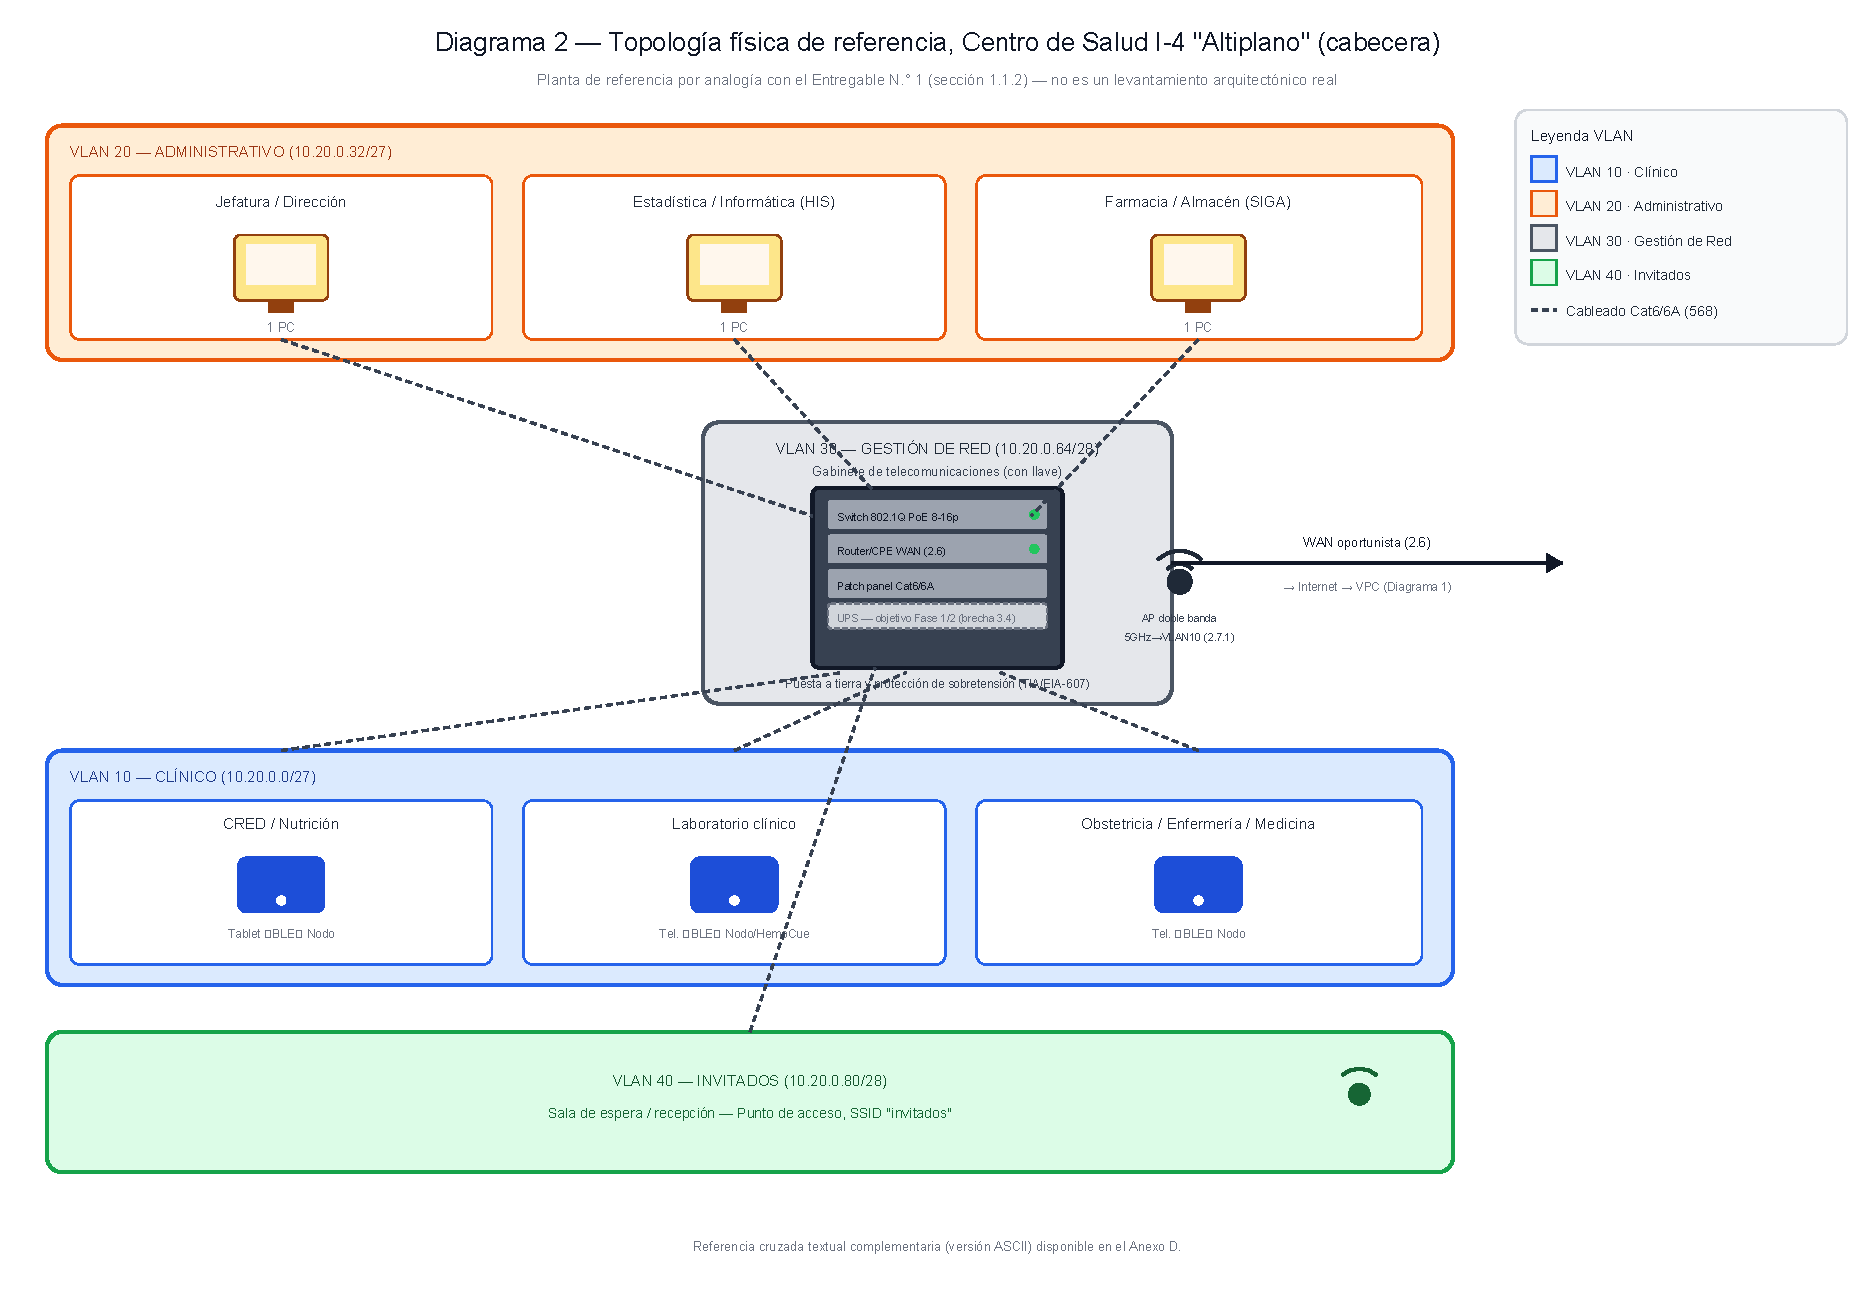
\includegraphics[width=0.88\linewidth,keepaspectratio]{assets/07-diseno-red/diagrama-02-topologia-fisica-cabecera.pdf}}
\caption{Diagrama 2 --- Topología física de referencia, Centro de Salud I-4 ``Altiplano'' (cabecera)}
\end{figure}

\textbf{Diagrama 2 --- Topología física de referencia, Centro de Salud I-4 ``Altiplano'' (cabecera).} Distribución de ambientes por VLAN (10 Clínico, 20 Administrativo, 30 Gestión de Red, 40 Invitados), gabinete de telecomunicaciones central y punto de acceso de doble banda.

Cuatro decisiones de diseño físico se explican a partir de este diagrama. Primero, el \textbf{gabinete de telecomunicaciones se ubica en posición central}, minimizando el cableado horizontal, conforme a la recomendación de TIA/EIA-569 de mantener distancias bajo 90 m (sin ser, a esta escala, un desafío real). Segundo, el gabinete se especifica \textbf{con cierre con llave}, control físico alineado con RNF-06/RNF-07 y con el principio de confidencialidad del Código ACM (sección 4.5). Tercero, se recomienda un \textbf{punto de acceso de doble banda (2.4/5 GHz)} en la zona clínica, priorizando 5 GHz para la VLAN 10 por menor congestión e interferencia con el enlace BLE nodo-teléfono (RQ-RED-12, sección 2.7.1). Cuarto, el punto de acceso de la sala de espera (SSID invitados, VLAN 40) atiende visitas de la DIRESA/GERESA, cooperación o soporte técnico externo, sin exponerlos en ningún momento a la VLAN clínica o administrativa.

\subsection{2.5 Topología física simplificada --- Puestos de Salud I-1/I-2}\label{topologuxeda-fuxedsica-simplificada-puestos-de-salud-i-1i-2}

El \textbf{Diagrama 3}, también producido con herramienta de diagramación vectorial, contrasta deliberadamente con el Diagrama 2 e ilustra por qué \textbf{no se justifica} replicar el esquema completo de 5 VLAN en este tipo de establecimiento: con un único dispositivo con app y un nodo rotativo, una segmentación 802.1Q completa añadiría costo y complejidad de gestión sin un beneficio de seguridad proporcional. La versión ASCII equivalente se conserva en el Anexo D.

\begin{figure}[H]
\centering
\pandocbounded{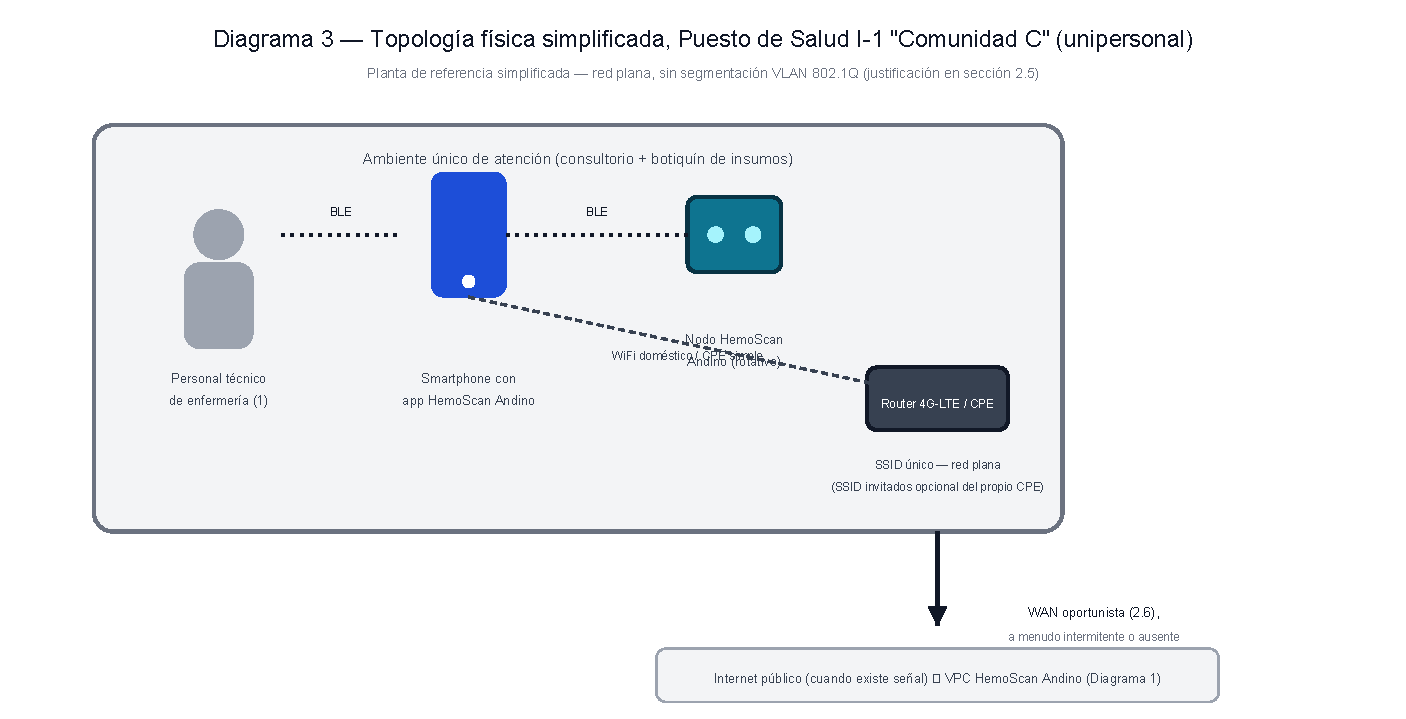
\includegraphics[width=0.88\linewidth,keepaspectratio]{assets/07-diseno-red/diagrama-03-topologia-fisica-puesto-salud.pdf}}
\caption{Diagrama 3 --- Topología física simplificada, Puesto de Salud I-1 ``Comunidad C'' (unipersonal)}
\end{figure}

\textbf{Diagrama 3 --- Topología física simplificada, Puesto de Salud I-1 ``Comunidad C'' (unipersonal).} Red plana sin VLAN 802.1Q; enlace BLE nodo-teléfono y salida WAN oportunista vía CPE doméstico.

Los Puestos de Salud I-2 (2 personas, ``Comunidad A''/``B'') siguen el mismo patrón simplificado, con la diferencia de que el CPE doméstico sirve a dos dispositivos en lugar de uno. Sigue sin justificarse una VLAN 802.1Q dedicada, pero si el propio CPE de bajo costo ofrece ``red de invitados'' integrada (común incluso en routers domésticos económicos), se recomienda activarla como control mínimo de aislamiento cuando personal externo visite el puesto, sin adquirir equipamiento adicional.

\subsection{2.6 Red WAN regional y enlace con la DIRESA}\label{red-wan-regional-y-enlace-con-la-diresa}

El \textbf{Diagrama 4} ilustra la red de área amplia que conecta los 7 establecimientos con el backend en la nube y, a través de este, con la Jefatura de microred, la DIRESA/GERESA y los sistemas nacionales:

\textbf{Diagrama 4 --- Red WAN regional en estrella (postas -\textgreater{} nube -\textgreater{} DIRESA/HIS-MINSA).}

\begin{samepage}\begin{verbatim}
   C.S. I-4 Altiplano        P.S. I-2 "A"/"B"          P.S. I-1 "C/D/E/F"
   (cabecera)                (2 postas)                (4 postas)
        \                         \                          /
         \   HTTPS/TLS, oportunista, sin enlace directo entre postas (RF-19, ADR-01)  /
          \_______________________  ________________________  ______________________/
                                  \/
                         INTERNET PÚBLICO (variable por establecimiento)
                                  |
                                  v
                  VPC HemoScan Andino — Backend FHIR (Diagrama 1, sección 2.2.2)
                                  |
                    +-------------+------------------------------+
                    v             v                              v
        Navegador — Jefatura   Navegador — Analista        Sistemas externos:
        de microred (HTTPS)    DIRESA/GERESA (HTTPS)       HIS-MINSA, Padrón Nominal,
                                                             SIGA (integración diferida, RF-30)
\end{verbatim}\end{samepage}

Un punto merece explicación aparte: el alcance solicitado incluye un ``enlace posta\textless-\textgreater DIRESA''. Del diagrama se desprende que \textbf{no existe un enlace de red dedicado y directo} entre la posta y la DIRESA/GERESA: la Jefatura y el analista acceden a la plataforma web como cualquier cliente de internet, autenticados vía Keycloak (RNF-06), sin VPN site-to-site ni red privada compartida --- consistente con el diagrama de despliegue del Entregable N.° 5 (sección 3.3).

Existe, sin embargo, un segundo significado que sí amerita diseño explícito: el \textbf{canal de interoperabilidad de sistema a sistema} con HIS-MINSA/Padrón Nominal (RF-30), probablemente sujeto a una política propia del MINSA/DIRESA (restricción de IP de origen, VPN dedicada, o un gateway nacional de interoperabilidad) --- \textbf{{[}DATO PENDIENTE DE VALIDAR: mecanismo y política de conectividad exacta exigida por MINSA/DIRESA; no disponible hasta un acercamiento institucional formal{]}}. Se recomienda evaluar en Fase 1 un túnel IPsec site-to-site o una VPN dedicada exclusivamente para este canal, como defensa en profundidad adicional a TLS.

Respecto de las opciones de enlace WAN por posta, en orden de preferencia:

\begin{enumerate}
\def\labelenumi{\arabic{enumi}.}
\tightlist
\item
  \textbf{Primario --- 4G/LTE celular.} Router/CPE con SIM de un operador móvil con cobertura en la zona --- \textbf{{[}DATO PENDIENTE DE VALIDAR: operador y nivel de señal real en la ubicación exacta de cada establecimiento{]}}. Es, en general, la alternativa más económica y de despliegue más simple para zonas rurales altoandinas con alguna cobertura celular.
\item
  \textbf{Secundario/contingencia --- VSAT o servicio satelital de nueva generación} (constelaciones de órbita baja). Alternativa a evaluar para establecimientos sin cobertura celular o como respaldo del enlace primario --- \textbf{{[}DATO PENDIENTE DE VALIDAR: disponibilidad, cobertura y costo real de un proveedor satelital en la ubicación exacta de la microred{]}}.
\item
  \textbf{Última instancia --- sincronización manual (``modo desconectado extendido'').} Cuando ninguna opción anterior esté disponible de forma sostenida, ADR-01 tolera que el personal traslade físicamente el teléfono hacia un punto con señal para vaciar la cola de sincronización; alternativa manual pero arquitectónicamente válida, coherente con la dispersión geográfica diagnosticada (Entregable N.° 1) y con que RF-19/RNF-17 no impongan un límite de tiempo al restablecimiento de la conectividad.
\end{enumerate}

\subsection{2.7 Protocolos y seguridad por segmento}\label{protocolos-y-seguridad-por-segmento}

\subsubsection{2.7.1 Enlace BLE nodo-teléfono}\label{enlace-ble-nodo-teluxe9fono}

El nodo opera como periférico BLE (rol GATT \emph{server}) y el teléfono como central (rol GATT \emph{client}), en relación estrictamente uno a uno por captura, nunca en malla. Ante la ausencia de pantalla o teclado en el ESP32-S3, el mecanismo de emparejamiento más viable es ``Just Works'', que no ofrece protección plena contra ataques de intermediario (MITM); se mitiga mediante controles compensatorios: exigencia de proximidad física real durante el emparejamiento (el propio flujo clínico ya la requiere), ventanas de emparejamiento breves, y el hecho de que el dato transmitido (señales ópticas crudas, sin identificación directa del paciente en el payload BLE) tiene un valor de explotación limitado si fuera interceptado de forma aislada. Se recomienda evaluar, en la siguiente iteración del firmware (paquete EDT 4.3), el uso de \emph{LE Secure Connections} con \emph{bonding} si el stack BLE del ESP32-S3 lo soporta de forma estable --- \textbf{{[}DATO PENDIENTE DE VALIDAR: si el firmware implementará bonding persistente o pairing por sesión; corresponde conjuntamente a los Integrantes 1 y 3{]}}. Para minimizar la interferencia mutua en la banda de 2.4 GHz, se recomienda que el punto de acceso de la VLAN 10 priorice la banda de 5 GHz para el tráfico de la app (sección 2.4), dejando la banda de 2.4 GHz más despejada para el enlace BLE.

\subsubsection{2.7.2 Sincronización app-backend}\label{sincronizaciuxf3n-app-backend}

Toda comunicación entre la app y el backend se realiza mediante HTTPS (TLS 1.2+, RNF-05), con los recursos FHIR transmitidos como \emph{bundles} transaccionales identificados por un UUID generado en el cliente (ADR-01), lo que permite al backend detectar y descartar reintentos duplicados sin perder ninguna determinación clínica. La red no requiere sesiones persistentes ni de baja latencia: cada sincronización es un conjunto de peticiones HTTP POST idempotentes completables en una ventana de conectividad breve e intermitente.

Se recomienda, como buena práctica compatible con el bajo presupuesto de Fase 0, un esquema simple de \textbf{calidad de servicio (QoS)} en el router de la cabecera que priorice el tráfico marcado como clínico (VLAN 10, puerto 443) por encima del de la VLAN 40 (Invitados) en el enlace WAN compartido, mediante marcado DSCP ---funcionalidad habitualmente disponible incluso en routers/CPE de gama baja, sin costo adicional significativo.

\subsubsection{2.7.3 Red LAN/WiFi interna}\label{red-lanwifi-interna}

La red interna de la cabecera opera sobre Ethernet (IEEE 802.3, cableado Cat6/6A) para los puestos fijos y sobre WiFi (IEEE 802.11, doble banda recomendada) para los dispositivos móviles clínicos, con cifrado WPA2-AES como mínimo aceptable y WPA3-Personal como meta, según la compatibilidad del parque de dispositivos de gama baja/media del personal de salud (Restricción 11, Entregable N.° 5). Cada SSID se asocia de forma unívoca a una única VLAN (sección 2.3), evitando el antipatrón de un solo SSID compartido entre perfiles de acceso distintos.

\subsubsection{2.7.4 Diseño para operación offline-first}\label{diseuxf1o-para-operaciuxf3n-offline-first}

Este principio transversal es la contribución de diseño de red más importante del documento: la red de HemoScan Andino \textbf{no está diseñada para eliminar la intermitencia de conectividad rural} (meta poco realista dado el contexto diagnosticado en el Entregable N.° 1), sino para \textbf{convivir con ella sin degradar la función clínica}. Se traduce en tres decisiones ya desarrolladas: (a) ninguna regla de negocio crítica depende de una llamada de red en tiempo real (RF-18, RNF-03); (b) la sincronización se ejecuta de forma oportunista, priorizada y con reintentos exponenciales, nunca bloqueante (RNF-17, ADR-01); y (c) el diseño físico y lógico de la red (secciones 2.1 a 2.6) reserva la dependencia de conectividad continua exclusivamente para las funciones no críticas (dashboard web, reportes agregados, interoperabilidad externa).

\begin{center}\rule{0.5\linewidth}{0.5pt}\end{center}

\section{3. Incorporación de Redundancia}\label{incorporaciuxf3n-de-redundancia}

\subsection{3.1 Análisis de puntos únicos de falla (SPOF)}\label{anuxe1lisis-de-puntos-uxfanicos-de-falla-spof}

La siguiente tabla identifica los puntos únicos de falla (\emph{Single Point of Failure}) de la red, su modo de falla, impacto, probabilidad cualitativa en Fase 0, y el nivel de redundancia efectivamente alcanzable hoy frente al objetivo de fases futuras. Es, deliberadamente, el punto del documento donde se declara con mayor honestidad la brecha entre lo deseable y lo presupuestalmente viable --- con una única excepción real ya incorporada, detallada en la fila de enlace WAN de la cabecera.

{\small
\begin{longtable}[]{@{}
  >{\raggedright\arraybackslash}p{(\linewidth - 12\tabcolsep) * \real{0.1429}}
  >{\raggedright\arraybackslash}p{(\linewidth - 12\tabcolsep) * \real{0.1429}}
  >{\raggedright\arraybackslash}p{(\linewidth - 12\tabcolsep) * \real{0.1429}}
  >{\raggedright\arraybackslash}p{(\linewidth - 12\tabcolsep) * \real{0.1429}}
  >{\raggedright\arraybackslash}p{(\linewidth - 12\tabcolsep) * \real{0.1429}}
  >{\raggedright\arraybackslash}p{(\linewidth - 12\tabcolsep) * \real{0.1429}}
  >{\raggedright\arraybackslash}p{(\linewidth - 12\tabcolsep) * \real{0.1429}}@{}}
\toprule\noalign{}
\begin{minipage}[b]{\linewidth}\raggedright
Componente
\end{minipage} & \begin{minipage}[b]{\linewidth}\raggedright
Modo de falla
\end{minipage} & \begin{minipage}[b]{\linewidth}\raggedright
Impacto
\end{minipage} & \begin{minipage}[b]{\linewidth}\raggedright
Probabilidad (Fase 0)
\end{minipage} & \begin{minipage}[b]{\linewidth}\raggedright
Mitigación aplicada en Fase 0
\end{minipage} & \begin{minipage}[b]{\linewidth}\raggedright
Redundancia Fase 0
\end{minipage} & \begin{minipage}[b]{\linewidth}\raggedright
Redundancia objetivo Fase 1/2
\end{minipage} \\
\midrule\noalign{}
\endhead
\bottomrule\noalign{}
\endlastfoot
Servidor único (backend + BD + Keycloak) & Caída de instancia, saturación de recursos, corrupción de base de datos & Bloquea sincronización, dashboard web y autenticación de sesiones nuevas; \textbf{no afecta} la captura/tamizaje offline (RNF-03) & Media (proveedor de nube de bajo costo, sin SLA contratado --- RNF-20 pendiente) & Respaldo automatizado diario de base de datos (sección 3.3) & Ninguna (instancia única) --- \textbf{riesgo residual aceptado explícitamente} & Instancia secundaria en espera (\emph{warm standby}) o servicio gestionado multi-zona \\
Enlace WAN --- cabecera & Corte de señal celular, saturación de la torre & Bloquea sincronización y acceso web; \textbf{no bloquea} captura/tamizaje (offline-first) & Alta (zona rural altoandina --- Debilidad D2) & \textbf{Router/CPE con doble SIM de dos operadores distintos (Anexo E, \textasciitilde=S/ 450) con conmutación automática} --- única medida de redundancia física de Fase 0 efectivamente presupuestada, condicionada al cierre de la brecha de financiamiento declarada en 3.4 & \textbf{Parcial} (dual-operador en un único router; sin diversidad de router físico) & Router dual con dos módems físicos independientes, o segundo enlace satelital \\
Enlace WAN --- puestos de salud I-1/I-2 & Corte de señal celular, saturación de la torre & Bloquea sincronización y acceso web; \textbf{no bloquea} captura (offline-first) & Alta (Debilidad D2) & Cola de reintentos exponenciales (RNF-17, ADR-01); operación offline \textgreater= 72 h (RNF-03) & Ninguna --- un solo proveedor/tecnología, por no justificarse el costo de un CPE dual-SIM en establecimientos de 1-2 dispositivos & Evaluar dual-SIM solo si el costo unitario baja en Fase 1/2 \\
Suministro eléctrico de la posta & Corte de energía, frecuente en zona altoandina & Apaga router/AP/switch; interrumpe el ciclo de captura si el nodo/teléfono se descargan & Alta (Debilidad D2) & Buffer local del nodo (RF-05, \textgreater= 50 capturas) y batería propia del teléfono & Sin UPS presupuestado (brecha declarada, sección 3.4) & UPS de 30-60 min mínimo para el equipo de red crítico de la cabecera \\
Switch/AP de la cabecera & Falla de hardware, sobrecalentamiento & Pérdida de LAN/WiFi interna en la cabecera & Baja-Media & Ninguna (equipo único); reemplazo manual reactivo & Ninguna & Equipo de repuesto en almacén (\emph{cold spare}) o AP secundario con solapamiento de cobertura \\
Nodo HemoScan Andino (hardware) & Falla de sensor, de batería o del módulo BLE & Imposibilidad de captura en el punto de atención específico & Media (3 nodos totales, sin unidad de respaldo dedicada por establecimiento) & Rotación operativa de los 3 nodos entre brigadas (EDT 2.4/2.5); el buffer local no se pierde ante el cambio de nodo & Parcial (rotación operativa, no redundancia técnica 1:1) & Un nodo de respaldo adicional por microred activa en Fase 1 \\
Acceso web de la Jefatura/DIRESA & Corte de internet en cualquiera de los dos extremos & Imposibilidad de consulta en tiempo real del dashboard/mapa de cobertura & Media-Alta & Reportes exportables en PDF/CSV como canal alterno asíncrono (RF-36) & Sin alternativa en tiempo real & Posible acuerdo de conectividad reforzada con DIRESA en Fase 1/2 \\
\end{longtable}
}

\subsection{3.2 Alta disponibilidad por capas}\label{alta-disponibilidad-por-capas}

La siguiente tabla desagrega la estrategia de alta disponibilidad por capa, con objetivos ilustrativos de \textbf{RPO} y \textbf{RTO}, explícitamente etiquetados como metas de diseño y no como compromisos contractuales de un SLA (RNF-20 sigue pendiente de validar):

{\small
\begin{longtable}[]{@{}
  >{\raggedright\arraybackslash}p{(\linewidth - 8\tabcolsep) * \real{0.2000}}
  >{\raggedright\arraybackslash}p{(\linewidth - 8\tabcolsep) * \real{0.2000}}
  >{\raggedright\arraybackslash}p{(\linewidth - 8\tabcolsep) * \real{0.2000}}
  >{\raggedright\arraybackslash}p{(\linewidth - 8\tabcolsep) * \real{0.2000}}
  >{\raggedright\arraybackslash}p{(\linewidth - 8\tabcolsep) * \real{0.2000}}@{}}
\toprule\noalign{}
\begin{minipage}[b]{\linewidth}\raggedright
Capa
\end{minipage} & \begin{minipage}[b]{\linewidth}\raggedright
Estrategia de alta disponibilidad (Fase 0)
\end{minipage} & \begin{minipage}[b]{\linewidth}\raggedright
RPO ilustrativo
\end{minipage} & \begin{minipage}[b]{\linewidth}\raggedright
RTO ilustrativo
\end{minipage} & \begin{minipage}[b]{\linewidth}\raggedright
Estrategia objetivo (Fase 1/2)
\end{minipage} \\
\midrule\noalign{}
\endhead
\bottomrule\noalign{}
\endlastfoot
Cliente (app móvil) & Local-first + \emph{outbox} (ADR-01): el dispositivo es la fuente de verdad hasta la sincronización & 0 (no hay pérdida: los datos persisten localmente) & No aplica --- la app sigue plenamente operativa sin el servidor & Se mantiene igual; es el patrón más maduro de todo el diseño \\
Red LAN/WiFi (cabecera) & Un único punto de acceso, ubicación central & No aplica & Horas (reemplazo manual) & Segundo AP con solapamiento de cobertura \\
Red WAN --- cabecera & Router dual-SIM (dos operadores), conmutación automática (Anexo E) & Segundos a minutos (conmutación entre SIM) & Minutos, sujeto a la cobertura del operador secundario & Router dual con dos módems físicos independientes \\
Red WAN --- puestos I-1/I-2 & Un único enlace (4G u otro, según validación de campo) + cola de reintentos & Hasta 72 h de operación offline tolerada (RNF-03) & Depende del restablecimiento del operador (fuera de control del equipo) & Enlace dual (\emph{multi-WAN}) si el costo lo permite \\
Servidor (backend + BD + Keycloak) & Instancia única + respaldo diario automatizado & Hasta 24 h (ventana ilustrativa entre respaldos) & Hasta 48 h (tiempo ilustrativo de restauración manual) & Instancia secundaria o servicio gestionado multi-zona \\
\end{longtable}
}

El \textbf{Diagrama 5} resume estas rutas de redundancia y contingencia, distinguiendo lo que existe en Fase 0 de lo que es objetivo de fases posteriores:

\textbf{Diagrama 5 --- Rutas de redundancia y failover (Fase 0 vigente vs.~objetivo Fase 1/2).}

\begin{samepage}\begin{verbatim}
Cliente (app móvil)
  +- Ruta primaria (Fase 0): WiFi de la posta -> Internet -> Backend (nube)
  +- Ruta de contingencia (Fase 0, si aplica): datos móviles propios del teléfono del
  |  personal de salud, cuando exista SIM personal disponible -> Internet -> Backend
  +- Ruta última (Fase 0, siempre disponible): operación 100 % offline hasta 72 h
     continuas (RNF-03) + sincronización manual al desplazarse a un punto con señal

Posta — cabecera (router/CPE)
  +- Ruta primaria (Fase 0): Operador A vía SIM 1 del router dual-SIM (Anexo E)
  +- Ruta secundaria (Fase 0, conmutación automática): Operador B vía SIM 2 del mismo
     router — [DATO PENDIENTE DE VALIDAR: cierre de la brecha de financiamiento, sección 3.4]

Posta — puestos I-1/I-2 (router/CPE)
  +- Ruta primaria (Fase 0): un solo operador 4G/LTE — [DATO PENDIENTE DE VALIDAR: operador]
  +- Ruta objetivo (Fase 1/2): segundo operador o enlace satelital, router multi-WAN

Servidor (nube)
  +- Ruta primaria (Fase 0): instancia única + respaldo diario (sección 3.3)
  +- Ruta objetivo (Fase 1/2): instancia secundaria o servicio gestionado
     multi-zona, con conmutación por balanceador o DNS de failover
\end{verbatim}\end{samepage}

\subsection{3.3 Plan de contingencia y recuperación ante desastres}\label{plan-de-contingencia-y-recuperaciuxf3n-ante-desastres}

Se documenta a continuación un plan de contingencia básico (\emph{runbook}), suficiente para el alcance de la Fase 0, con escenario, mecanismo de detección, respuesta inmediata y responsable:

{\small
\begin{longtable}[]{@{}
  >{\raggedright\arraybackslash}p{(\linewidth - 8\tabcolsep) * \real{0.2000}}
  >{\raggedright\arraybackslash}p{(\linewidth - 8\tabcolsep) * \real{0.2000}}
  >{\raggedright\arraybackslash}p{(\linewidth - 8\tabcolsep) * \real{0.2000}}
  >{\raggedright\arraybackslash}p{(\linewidth - 8\tabcolsep) * \real{0.2000}}
  >{\raggedright\arraybackslash}p{(\linewidth - 8\tabcolsep) * \real{0.2000}}@{}}
\toprule\noalign{}
\begin{minipage}[b]{\linewidth}\raggedright
Escenario
\end{minipage} & \begin{minipage}[b]{\linewidth}\raggedright
Detección
\end{minipage} & \begin{minipage}[b]{\linewidth}\raggedright
Respuesta inmediata
\end{minipage} & \begin{minipage}[b]{\linewidth}\raggedright
Responsable
\end{minipage} & \begin{minipage}[b]{\linewidth}\raggedright
Referencia cruzada
\end{minipage} \\
\midrule\noalign{}
\endhead
\bottomrule\noalign{}
\endlastfoot
Corte de energía en la posta & Reporte del personal / pérdida de señal del AP & Continuar el tamizaje con la batería del teléfono/nodo; posponer la sincronización & Personal de salud / Integrante 1 (soporte remoto) & RF-18, RNF-03; EDT 2.5 \\
Caída del enlace WAN & La cola de sincronización agota reintentos sin conectar & La app continúa operando offline; reintento automático con retroceso exponencial & App móvil (automático); Integrante 1 (diagnóstico si es prolongado) & RNF-17, ADR-01 \\
Caída del servidor/backend & Verificación de disponibilidad (\emph{healthcheck} HTTP) o reporte de la Jefatura sobre imposibilidad de acceder al dashboard & Ejecutar el procedimiento de reinicio de la instancia; restaurar desde el respaldo más reciente si es necesario & Integrante 1 & EDT 2.2; sección 3.1 \\
Falla de un nodo de hardware & El personal reporta que el nodo no enciende o no logra emparejarse & Rotar hacia uno de los otros 2 nodos disponibles (EDT 2.4/2.5); registrar la incidencia en la bitácora de campo & Personal de salud / Integrante 1 & EDT 2.5 (bitácora de incidencias, disponibilidad \textgreater= 90 \% de las jornadas de campo) \\
Sospecha de incidente de seguridad (acceso no autorizado) & Alerta del propio Keycloak o revisión de los recursos AuditEvent & Revocar credenciales comprometidas; revisar trazas de auditoría; notificar conforme al protocolo de la Ley N.° 29733 & Integrante 1 (técnico) / Integrante 2 (gestión y comunicación) & RNF-06, RNF-07, RF-31, RN-11 \\
\end{longtable}
}

La política de respaldo de Fase 0 consiste en una copia automatizada diaria de PostgreSQL/PostGIS hacia un almacenamiento distinto al de la instancia primaria, retenida un mínimo razonable de 30 días --- \textbf{{[}DATO PENDIENTE DE VALIDAR: política exacta de retención y mecanismo de respaldo del proveedor de nube finalmente elegido{]}}. Es modesta frente a un esquema activo-activo, pero consistente con el riesgo aceptado en 3.1 y con que ninguna función clínica crítica dependa de la disponibilidad continua del servidor.

\subsection{3.4 Brecha presupuestal de redundancia y hoja de ruta por fases}\label{brecha-presupuestal-de-redundancia-y-hoja-de-ruta-por-fases}

El presupuesto validado de Fase 0 (S/ 3,124) no contiene una partida específica para equipamiento de red más allá del rubro ``servidor/nube'' (S/ 320, EDT 2.2). Frente a esta restricción, el equipo adopta una única medida correctiva concreta y presupuestada dentro de la propia estimación referencial del Anexo E: el \textbf{router/CPE 4G-LTE con doble SIM} (\textasciitilde=S/ 450) se recomienda como el equipo WAN de la cabecera desde la propia Fase 0 ---y no como un ítem diferido a Fase 1/2, como se planteaba en una versión anterior de este documento---, porque el sobrecosto frente a un router de SIM única (\textasciitilde=S/ 200-250) es marginal y porque, de todas las capas analizadas en 3.1, es la que ofrece la relación costo-beneficio de redundancia más alta.

Ese ítem, sin embargo, \textbf{no está cerrado financieramente}: la partida de contingencia del 10 \% del presupuesto validado (S/ 284) no cubre el costo íntegro de S/ 450, dejando un diferencial de aproximadamente \textbf{S/ 166} --- \textbf{{[}DATO PENDIENTE DE VALIDAR: fuente de financiamiento del diferencial; opciones no excluyentes son un aporte de contraparte de la microred/DIRESA anfitriona, una reasignación menor dentro de la línea base del Entregable N.° 3, o una ampliación presupuestal formal{]}}. Hasta que ese diferencial se cierre, la redundancia de enlace WAN de la cabecera se mantiene como una recomendación de diseño fuertemente respaldada, no como una redundancia ya garantizada --- distinción que la tabla 3.1 refleja explícitamente.

El resto del equipamiento del Anexo E (switch, puntos de acceso, cableado, UPS; \textasciitilde=S/ 1,280 adicionales) permanece sin fuente de financiamiento identificada. La hoja de ruta de cierre de esa brecha mayor sigue siendo la proyección de hosting de Fase 1 (\textasciitilde=S/ 1,200/año, Entregable N.° 2), que ya contempla un salto de escala coherente con presupuestar entonces un proveedor de nube multi-zona y el equipamiento de red hoy pendiente.

\begin{center}\rule{0.5\linewidth}{0.5pt}\end{center}

\section{4. Cumplimiento de Estándares}\label{cumplimiento-de-estuxe1ndares}

\subsection{4.1 Estándares de cableado estructurado}\label{estuxe1ndares-de-cableado-estructurado}

{\small
\begin{longtable}[]{@{}
  >{\raggedright\arraybackslash}p{(\linewidth - 4\tabcolsep) * \real{0.3333}}
  >{\raggedright\arraybackslash}p{(\linewidth - 4\tabcolsep) * \real{0.3333}}
  >{\raggedright\arraybackslash}p{(\linewidth - 4\tabcolsep) * \real{0.3333}}@{}}
\toprule\noalign{}
\begin{minipage}[b]{\linewidth}\raggedright
Estándar
\end{minipage} & \begin{minipage}[b]{\linewidth}\raggedright
Ámbito
\end{minipage} & \begin{minipage}[b]{\linewidth}\raggedright
Aplicación en el diseño de HemoScan Andino
\end{minipage} \\
\midrule\noalign{}
\endhead
\bottomrule\noalign{}
\endlastfoot
TIA/EIA-568-C (series) / ISO/IEC 11801 & Cableado de telecomunicaciones para edificios comerciales & Cableado horizontal Cat6/Cat6A recomendado para la cabecera (Diagrama 2), con margen de desempeño para un eventual salto a mayores velocidades en Fase 2; conectorización RJ-45 bajo esquema T568B \\
TIA/EIA-569-D & Rutas y espacios para telecomunicaciones & Gabinete de telecomunicaciones de pequeño formato en la cabecera, canalización protegida frente a polvo/humedad, y distancias de cableado horizontal dentro del límite convencional de 90 m \\
TIA/EIA-606-B & Administración de la infraestructura de telecomunicaciones (etiquetado y documentación) & Esquema de etiquetado propuesto para puertos de switch, cables y VLAN, con convención {[}Sitio{]}-{[}Ambiente{]}-{[}Consecutivo{]} y ejemplo aplicado al patch panel de la cabecera (Anexo D), que permite a cualquier técnico de soporte ---incluyendo personal nuevo, dada la alta rotación por el régimen SERUMS diagnosticada en el Entregable N.° 1--- identificar sin ambigüedad cualquier punto de la red \\
TIA/EIA-607-D & Puesta a tierra y enlace equipotencial & Puesta a tierra del gabinete y protección contra sobretensión, dado el riesgo de tormentas eléctricas del altiplano a 3,800 m s. n.~m. y la inestabilidad eléctrica ya diagnosticada (Debilidad D2) \\
TIA-942 (referencia parcial) & Infraestructura de centros de datos & No aplica directamente en Fase 0, al alojarse el backend en un proveedor de nube pública; se cita como referencia solo si una fase futura contemplara un centro de datos propio o de la DIRESA \\
\end{longtable}
}

\subsection{4.2 Estándares IEEE 802.x}\label{estuxe1ndares-ieee-802.x}

{\small
\begin{longtable}[]{@{}
  >{\raggedright\arraybackslash}p{(\linewidth - 6\tabcolsep) * \real{0.2500}}
  >{\raggedright\arraybackslash}p{(\linewidth - 6\tabcolsep) * \real{0.2500}}
  >{\raggedright\arraybackslash}p{(\linewidth - 6\tabcolsep) * \real{0.2500}}
  >{\raggedright\arraybackslash}p{(\linewidth - 6\tabcolsep) * \real{0.2500}}@{}}
\toprule\noalign{}
\begin{minipage}[b]{\linewidth}\raggedright
Estándar
\end{minipage} & \begin{minipage}[b]{\linewidth}\raggedright
Ámbito
\end{minipage} & \begin{minipage}[b]{\linewidth}\raggedright
Aplicación específica en HemoScan Andino
\end{minipage} & \begin{minipage}[b]{\linewidth}\raggedright
Elemento(s) de red
\end{minipage} \\
\midrule\noalign{}
\endhead
\bottomrule\noalign{}
\endlastfoot
IEEE 802.3 / 802.3u / 802.3ab (Ethernet, Fast Ethernet, Gigabit sobre par trenzado) & Cableado LAN & Backbone y cableado horizontal de la cabecera; puertos de switch a 1000 Mbps como mínimo recomendado & Switch, patch panel, cableado horizontal (Diagrama 2) \\
IEEE 802.3af (PoE) / 802.3at (PoE+) & Alimentación eléctrica sobre Ethernet & Alimentación de los puntos de acceso WiFi desde un switch, mitigando parcialmente los cortes eléctricos frecuentes (Debilidad D2) sin tendido eléctrico adicional & Switch PoE, puntos de acceso \\
IEEE 802.11 (WiFi), en particular 802.11n/ac de doble banda & Red inalámbrica local & SSID mapeados 1:1 a las VLAN 10/20/30/40 de la cabecera (sección 2.3); banda de 5 GHz priorizada para tráfico clínico (sección 2.7.1) & Puntos de acceso, dispositivos móviles/tablets \\
IEEE 802.1Q & Etiquetado de VLAN (\emph{trunking}) & Enlace troncal switch\textless-\textgreater router/firewall que transporta las 5 VLAN de la cabecera sobre un único enlace físico & Switch, router/firewall \\
IEEE 802.1X & Control de acceso a la red basado en puertos (NAC) & Recomendado para la VLAN 20 en Fase 1/2, integrado conceptualmente con Keycloak (ADR-09); en Fase 0 se acepta un control más simple (filtrado por MAC/contraseña robusta) por restricción de presupuesto --- \textbf{brecha declarada explícitamente} & Switch, controlador de acceso \\
IEEE 802.1D (STP) / 802.1w (RSTP) & Prevención de bucles de capa 2 & Aplicable si la cabecera incorpora un segundo switch en Fase 1/2 (sección 3.2); no requerido con el switch único de Fase 0 & Switches (topología con más de un nodo de capa 2) \\
IEEE 802.11i (WPA2) / WPA3 & Seguridad de la capa de enlace inalámbrica & Cifrado obligatorio en las 4 VLAN inalámbricas de la cabecera; WPA3-Personal como meta, WPA2-AES como mínimo aceptable dado el parque de dispositivos de gama baja/media & Puntos de acceso, dispositivos móviles \\
Familia IEEE 802.15 (WPAN) --- referencia histórica de Bluetooth & Redes de área personal inalámbricas & El enlace nodo\textless-\textgreater teléfono opera sobre BLE, hoy gobernado por el Bluetooth SIG y no por el IEEE, aunque originado dentro de la familia WPAN 802.15; se cita por completitud, no como certificación IEEE vigente sobre BLE & Nodo HemoScan Andino, módulo BLE del teléfono \\
\end{longtable}
}

\subsection{4.3 Cumplimiento normativo sectorial}\label{cumplimiento-normativo-sectorial}

{\small
\begin{longtable}[]{@{}
  >{\raggedright\arraybackslash}p{(\linewidth - 4\tabcolsep) * \real{0.3333}}
  >{\raggedright\arraybackslash}p{(\linewidth - 4\tabcolsep) * \real{0.3333}}
  >{\raggedright\arraybackslash}p{(\linewidth - 4\tabcolsep) * \real{0.3333}}@{}}
\toprule\noalign{}
\begin{minipage}[b]{\linewidth}\raggedright
Norma
\end{minipage} & \begin{minipage}[b]{\linewidth}\raggedright
Exigencia relevante para la red
\end{minipage} & \begin{minipage}[b]{\linewidth}\raggedright
Control de red aplicado
\end{minipage} \\
\midrule\noalign{}
\endhead
\bottomrule\noalign{}
\endlastfoot
Ley N.° 29733 (Protección de Datos Personales) & Minimización, seguridad y confidencialidad de datos de salud de menores de edad (RNF-07, RNF-19) & Segmentación VLAN 10 Clínico aislada de VLAN 40 Invitados y VLAN 20 Administrativo (sección 2.3); cifrado TLS 1.2+ en tránsito (RNF-05); acceso administrativo restringido a VLAN 20/30 \\
DS 115-2025-PCM (reglamento de IA, Ley N.° 31814) & Trazabilidad y supervisión humana de sistemas de IA en salud; registro auditable de toda inferencia (RNF-08, RNF-18) & Sincronización horaria (NTP) obligatoria en todos los puntos de captura y registro (sección 4.3.1); disponibilidad suficiente para no bloquear la auditoría posterior, sin comprometer la operación offline crítica \\
NTS 213-MINSA/DGIESP-2024 & Continuidad del proceso de tamizaje y consejería (no impone requisitos de red directos) & Diseño offline-first que no condiciona la atención clínica a la disponibilidad de conectividad (sección 2.7.4) \\
OSIPTEL (regulación peruana de telecomunicaciones) & Uso del espectro radioeléctrico & WiFi (802.11) y BLE (2.4 GHz) operan en bandas no licenciadas; no se requiere trámite ante OSIPTEL. El enlace 4G/LTE opera bajo el espectro licenciado del operador contratado como servicio, sin trámite propio de HemoScan Andino \\
\end{longtable}
}

\subsubsection{4.3.1 Sincronización horaria (NTP) como requisito silencioso de auditabilidad}\label{sincronizaciuxf3n-horaria-ntp-como-requisito-silencioso-de-auditabilidad}

Se destaca un requisito fácil de omitir pero indispensable para el DS 115-2025-PCM: la integridad de los recursos FHIR Provenance/AuditEvent (RF-31, RNF-08) depende de que las marcas de tiempo del nodo, el teléfono y el backend sean \textbf{consistentes entre sí}. Si los relojes se desincronizan (escenario plausible en dispositivos de gama baja/media sin mantenimiento regular), la secuencia auditable de ``qué ocurrió primero'' ---captura, inferencia, corrección por altitud, confirmación clínica--- podría volverse ambigua, debilitando exactamente la trazabilidad exigida. Se recomienda que el backend en la nube ejecute un cliente NTP estándar sincronizado contra servidores de tiempo confiables, y que la app móvil registre, junto a cada marca de tiempo local, un indicador de la última sincronización horaria conocida del dispositivo, de modo que cualquier inconsistencia temporal sea, en sí misma, detectable y auditable en lugar de silenciosa.

\subsection{4.4 Matriz consolidada de cumplimiento}\label{matriz-consolidada-de-cumplimiento}

{\small
\begin{longtable}[]{@{}
  >{\raggedright\arraybackslash}p{(\linewidth - 4\tabcolsep) * \real{0.3333}}
  >{\raggedright\arraybackslash}p{(\linewidth - 4\tabcolsep) * \real{0.3333}}
  >{\raggedright\arraybackslash}p{(\linewidth - 4\tabcolsep) * \real{0.3333}}@{}}
\toprule\noalign{}
\begin{minipage}[b]{\linewidth}\raggedright
Dimensión de cumplimiento
\end{minipage} & \begin{minipage}[b]{\linewidth}\raggedright
Estado en este diseño
\end{minipage} & \begin{minipage}[b]{\linewidth}\raggedright
Observación
\end{minipage} \\
\midrule\noalign{}
\endhead
\bottomrule\noalign{}
\endlastfoot
Cableado estructurado (TIA/EIA-568/569/606/607, ISO/IEC 11801) & Aplicado como diseño de referencia & Pendiente de validación con relevamiento de campo real \\
Redes de área local y personal (IEEE 802.3, 802.11, 802.15) & Aplicado & BLE gobernado hoy por Bluetooth SIG, no por IEEE (aclaración explícita en 4.2) \\
Segmentación y control de acceso (802.1Q, 802.1X) & 802.1Q aplicado plenamente; 802.1X diferido a Fase 1/2 & Brecha declarada explícitamente por restricción de presupuesto/capacidades de Fase 0 \\
Protección de datos personales (Ley N.° 29733) & Aplicado mediante segmentación, cifrado y control de acceso & Pendiente de dictamen de un comité de ética constituido (Entregable N.° 1) \\
Marco de IA en salud (DS 115-2025-PCM) & Aplicado mediante NTP, disponibilidad y no bloqueo de la supervisión humana & La responsabilidad principal de la trazabilidad de IA recae en el software (Entregable N.° 5); la red la habilita, no la reemplaza \\
Regulación de telecomunicaciones (OSIPTEL) & Cumplido por uso de bandas no licenciadas y de espectro licenciado de operador contratado & No se identifican trámites regulatorios propios pendientes para HemoScan Andino como organización \\
\end{longtable}
}

\subsection{4.5 Ética profesional en el diseño de red (Código de Ética y Conducta Profesional de la ACM)}\label{uxe9tica-profesional-en-el-diseuxf1o-de-red-cuxf3digo-de-uxe9tica-y-conducta-profesional-de-la-acm}

El diseño de una red que transporta datos de salud de menores de edad en un contexto de vulnerabilidad social y geográfica admite una lectura desde la ética profesional de la disciplina, para lo cual se adopta como referencia el \textbf{Código de Ética y Conducta Profesional de la ACM (2018)}. El principio \textbf{1.2 (``Evitar daño'')} se traduce en la segmentación VLAN que impide que un dispositivo de invitado comprometido alcance datos clínicos (sección 2.3), y en la declaración explícita ---no ocultamiento--- de los riesgos residuales de la Fase 0 (servidor único, ausencia de UPS, redundancia WAN condicionada a financiamiento) en la sección 3.1. El principio \textbf{1.6 (``Respetar la privacidad'')} se materializa en el aislamiento de la VLAN clínica y en la reserva de un segmento propio para el futuro canal de aprendizaje federado que nunca debe transportar datos crudos de pacientes (RN-09, sección 2.2.2). El principio \textbf{1.7 (``Honrar la confidencialidad'')} respalda el control de acceso físico al gabinete de telecomunicaciones (sección 2.4, Anexo D) y la restricción de la VLAN 30 a personal técnico autorizado.

El principio \textbf{2.5 (``Ofrecer evaluaciones exhaustivas de los sistemas informáticos y sus impactos, incluido el análisis de riesgos posibles'')} es, en esencia, el mandato que la sección 3 intenta cumplir: un análisis de puntos únicos de falla que no minimiza ni exagera el riesgo real de una arquitectura de Fase 0 deliberadamente austera. Se añade el principio \textbf{3.7 (``Reconocer y prestar especial atención a los sistemas que se integran en la infraestructura de la sociedad'')}: si HemoScan Andino avanza hacia la Fase 2 de escalamiento regional (Entregable N.° 2), su red dejará progresivamente de ser un proyecto de tesis para convertirse en infraestructura crítica de salud pública regional, responsabilidad que este diseño anticipa desde la Fase 0 mediante la escalabilidad del direccionamiento (sección 2.2) y la hoja de ruta de redundancia (sección 3.4), en lugar de postergarla para cuando la escala haga más costoso corregirla.

\begin{center}\rule{0.5\linewidth}{0.5pt}\end{center}

\section{Anexos}\label{anexos}

\subsection{Anexo A --- Glosario de términos técnicos de este entregable}\label{anexo-a-glosario-de-tuxe9rminos-tuxe9cnicos-de-este-entregable}

{\small
\begin{longtable}[]{@{}
  >{\raggedright\arraybackslash}p{(\linewidth - 2\tabcolsep) * \real{0.5000}}
  >{\raggedright\arraybackslash}p{(\linewidth - 2\tabcolsep) * \real{0.5000}}@{}}
\toprule\noalign{}
\begin{minipage}[b]{\linewidth}\raggedright
Término
\end{minipage} & \begin{minipage}[b]{\linewidth}\raggedright
Definición breve
\end{minipage} \\
\midrule\noalign{}
\endhead
\bottomrule\noalign{}
\endlastfoot
ACL (Access Control List) & Lista de control de acceso; conjunto de reglas que permiten o deniegan tráfico entre segmentos de red (sección 2.3) \\
BLE / GATT & Bluetooth Low Energy y su perfil de atributos genéricos (\emph{Generic Attribute Profile}), usado en el enlace nodo-teléfono \\
CIDR (Classless Inter-Domain Routing) & Notación de direccionamiento IP sin clases, usada para expresar subredes (p.~ej., /24, /27) \\
CPE (Customer Premises Equipment) & Equipo de telecomunicaciones instalado en las instalaciones del cliente (router/módem de la posta) \\
DMZ (Zona Desmilitarizada) & Segmento de red perimetral que aísla los recursos expuestos a internet de la red interna; reinterpretada en este documento como subred pública/privada de una VPC (sección 2.2.2) \\
DSCP & \emph{Differentiated Services Code Point}; campo usado para marcar y priorizar tráfico (calidad de servicio, sección 2.7.2) \\
IEEE 802.x & Familia de estándares del \emph{Institute of Electrical and Electronics Engineers} para redes de área local, personal y metropolitana (sección 4.2) \\
ISO/IEC 11801 & Estándar internacional de cableado estructurado, análogo a la serie TIA/EIA-568 \\
NAT & Traducción de direcciones de red; permite que múltiples dispositivos con IP privada compartan una IP pública \\
NTP (Network Time Protocol) & Protocolo de sincronización horaria entre dispositivos de red (sección 4.3.1) \\
OSIPTEL & Organismo Supervisor de Inversión Privada en Telecomunicaciones, regulador peruano del sector \\
PAN (Personal Area Network) & Red de área personal; en este proyecto, el enlace BLE nodo-teléfono \\
PoE / PoE+ & \emph{Power over Ethernet}; alimentación eléctrica de dispositivos de red a través del cable de datos (IEEE 802.3af/at) \\
QoS (Quality of Service) & Conjunto de técnicas para priorizar cierto tráfico de red sobre otro \\
RPO / RTO & \emph{Recovery Point Objective} / \emph{Recovery Time Objective}; métricas de tolerancia a pérdida de datos y a tiempo de interrupción (sección 3.2) \\
SPOF (Single Point of Failure) & Punto único de falla; componente cuya caída interrumpe el funcionamiento de todo el sistema que depende de él (sección 3.1) \\
SSID & Nombre de una red inalámbrica (\emph{Service Set Identifier}) \\
TIA/EIA & \emph{Telecommunications Industry Association} / \emph{Electronic Industries Alliance}; organismos que emiten estándares de cableado estructurado (sección 4.1) \\
VLAN (802.1Q) & Red de área local virtual; mecanismo de segmentación lógica de una misma red física, incluida su VLAN nativa (sección 2.3) \\
VLSM (Variable Length Subnet Masking) & Técnica de subnetting con máscaras de longitud variable, usada en el direccionamiento de la sección 2.2 \\
VPC (Virtual Private Cloud) & Red privada virtual dentro de un proveedor de nube pública, usada para alojar el backend de HemoScan Andino \\
VPN / IPsec & Red privada virtual y conjunto de protocolos para establecer túneles cifrados entre redes (sección 2.6) \\
VSAT & \emph{Very Small Aperture Terminal}; tecnología de conectividad satelital de bajo costo relativo \\
WAN (Wide Area Network) & Red de área amplia; en este proyecto, el enlace entre cada posta e internet/la nube \\
\end{longtable}
}

\subsection{Anexo B --- Fuentes y referencias}\label{anexo-b-fuentes-y-referencias}

\textbf{Fuentes normativas y científicas del proyecto} (ya citadas y validadas en los Entregables N.° 1, N.° 2, N.° 3 y N.° 5; reutilizadas aquí sin modificación):
- ENDES 2025 --- prevalencia de anemia infantil de 56.1 \% en menores de 3 años en Puno.
- Gonzales, G. F. et al.~(2025) --- riesgo de sobrediagnóstico por corrección de hemoglobina en altitud.
- Baquerizo-Sedano, L. et al.~(2025) --- íd., evidencia complementaria sobre corrección de hemoglobina por altitud.
- NTS 213-MINSA/DGIESP-2024 --- Norma Técnica de Salud para el manejo de la anemia.
- DS 115-2025-PCM --- reglamento de la Ley N.° 31814 de inteligencia artificial (salud como sector de alto riesgo, exige supervisión humana y trazabilidad).
- Ley N.° 29733 --- Ley de Protección de Datos Personales.

\textbf{Fuentes y estándares técnicos de referencia general de la industria} (no específicos de la organización ni verificados contra el territorio exacto de la microred ilustrativa; se citan como respaldo de las decisiones de diseño, no como mediciones de campo):
- Telecommunications Industry Association (TIA) --- serie de estándares TIA/EIA-568 (cableado), 569 (rutas y espacios), 606 (administración) y 607 (puesta a tierra).
- ISO/IEC 11801 --- estándar internacional de cableado estructurado.
- Institute of Electrical and Electronics Engineers (IEEE) --- estándares 802.3, 802.3af/at, 802.11, 802.1Q, 802.1X, 802.1D/w y familia 802.15 (WPAN).
- Bluetooth SIG --- especificación central de Bluetooth Low Energy (BLE), gobernanza actual del protocolo usado en el enlace nodo-teléfono.
- IETF RFC 1918 --- asignación de direccionamiento IPv4 privado.
- IETF --- Network Time Protocol (NTP), estándar de sincronización horaria.
- Documentación general de patrones de arquitectura de nube (VPC pública/privada), citada de forma genérica sin compromiso con un proveedor específico --- \textbf{{[}DATO PENDIENTE DE VALIDAR: proveedor de nube definitivo{]}}.
- ACM (Association for Computing Machinery) --- Código de Ética y Conducta Profesional (2018).
- OSIPTEL --- marco regulatorio peruano de telecomunicaciones y uso de espectro no licenciado.

\textbf{Documentos internos del propio proyecto HemoScan Andino} (insumo directo y obligatorio de este entregable):
- Entregable N.° 1 --- Diagnóstico Organizacional y Alineamiento Estratégico.
- Entregable N.° 2 --- Business Case.
- Entregable N.° 3 --- Plan de Gestión del Proyecto (EDT, presupuesto, riesgos).
- Entregable N.° 5 --- Requerimientos y Diseño del Sistema (SRS, arquitectura, ADR-01 a ADR-10).

\subsection{Anexo C --- Trazabilidad de requisitos de red}\label{anexo-c-trazabilidad-de-requisitos-de-red}

Para evitar duplicar el texto completo de cada requerimiento ---ya desarrollado en la sección 1.2.4--- este anexo condensa en una sola tabla la trazabilidad íntegra: identificador, prioridad MoSCoW, requisito no funcional/regla de negocio de origen (Entregable N.° 5) y elemento de diseño de este documento donde se resuelve. Esta tabla sustituye a los dos anexos de requisitos de la versión anterior de este documento (que reproducían, por separado y de forma redundante, el mismo contenido ya presentado en el cuerpo).

{\small
\begin{longtable}[]{@{}
  >{\raggedright\arraybackslash}p{(\linewidth - 6\tabcolsep) * \real{0.2500}}
  >{\raggedright\arraybackslash}p{(\linewidth - 6\tabcolsep) * \real{0.2500}}
  >{\raggedright\arraybackslash}p{(\linewidth - 6\tabcolsep) * \real{0.2500}}
  >{\raggedright\arraybackslash}p{(\linewidth - 6\tabcolsep) * \real{0.2500}}@{}}
\toprule\noalign{}
\begin{minipage}[b]{\linewidth}\raggedright
ID
\end{minipage} & \begin{minipage}[b]{\linewidth}\raggedright
Prioridad
\end{minipage} & \begin{minipage}[b]{\linewidth}\raggedright
RNF/RN de origen
\end{minipage} & \begin{minipage}[b]{\linewidth}\raggedright
Elemento de diseño
\end{minipage} \\
\midrule\noalign{}
\endhead
\bottomrule\noalign{}
\endlastfoot
RQ-RED-01 & Must & RF-01, RNF-02 & Sección 2.7.1 \\
RQ-RED-02 & Should & Sección 2.7.1 (capacidad de firmware pendiente) & Sección 2.7.1 \\
RQ-RED-03 & Must & RNF-03, RNF-17, ADR-01 & Secciones 2.7.4, 3.1, 3.2 \\
RQ-RED-04 & Must & RNF-05 & Secciones 2.2.2, 2.7.2 \\
RQ-RED-05 & Must & RNF-07, RNF-19 & Sección 2.3 \\
RQ-RED-06 & Should & RNF-12, ADR-02 & Sección 2.2.1 \\
RQ-RED-07 & Must & RNF-08, RF-31, DS 115-2025-PCM & Sección 4.3.1 \\
RQ-RED-08 & Should & RF-30 & Sección 2.6 \\
RQ-RED-09 & Should & RF-33 a RF-38 & Sección 2.6 \\
RQ-RED-10 & Must & Entregables N.° 2 y N.° 3 & Secciones 1.3.2, 3.4, Anexo E \\
RQ-RED-11 & Must & RF-05, Entregable N.° 1 (Debilidad D2) & Sección 2.7.4 \\
RQ-RED-12 & Should & RNF-02 & Sección 2.7.1 \\
RQ-RED-13 & Must & RNF-20 (pendiente), ADR-01, ADR-02 & Secciones 3.1, 3.2 \\
RQ-RED-14 & Could (Fase 1/2) & RN-09, ADR-08 & Sección 2.2.2 \\
\end{longtable}
}

\subsection{Anexo D --- Diagramas detallados}\label{anexo-d-diagramas-detallados}

Este anexo reúne tres elementos: (D.1) el índice de los seis diagramas del documento, numerados de forma consecutiva sin saltos; (D.2) la versión ASCII complementaria de los Diagramas 2 y 3, útil como referencia textual rápida frente a la versión gráfica vectorial ya presentada en las secciones 2.4 y 2.5; y (D.3) un diagrama de detalle que \textbf{no se muestra en el cuerpo del documento}: la elevación del rack del gabinete de telecomunicaciones con el esquema de etiquetado TIA/EIA-606-B, requerido por la sección 4.1 y no desarrollado hasta esta versión.

\subsubsection{D.1 Índice de diagramas}\label{d.1-uxedndice-de-diagramas}

{\small
\begin{longtable}[]{@{}
  >{\raggedright\arraybackslash}p{(\linewidth - 6\tabcolsep) * \real{0.2500}}
  >{\raggedright\arraybackslash}p{(\linewidth - 6\tabcolsep) * \real{0.2500}}
  >{\raggedright\arraybackslash}p{(\linewidth - 6\tabcolsep) * \real{0.2500}}
  >{\raggedright\arraybackslash}p{(\linewidth - 6\tabcolsep) * \real{0.2500}}@{}}
\toprule\noalign{}
\begin{minipage}[b]{\linewidth}\raggedright
Diagrama
\end{minipage} & \begin{minipage}[b]{\linewidth}\raggedright
Descripción
\end{minipage} & \begin{minipage}[b]{\linewidth}\raggedright
Formato
\end{minipage} & \begin{minipage}[b]{\linewidth}\raggedright
Ubicación
\end{minipage} \\
\midrule\noalign{}
\endhead
\bottomrule\noalign{}
\endlastfoot
Diagrama 1 & Topología lógica general de red, de extremo a extremo (nodo--teléfono--posta--nube--DIRESA) & Esquema lógico en texto & Sección 2.1 \\
Diagrama 2 & Topología física de referencia --- Centro de Salud I-4 ``Altiplano'' (cabecera), por VLAN & Gráfico vectorial (SVG) + ASCII complementario (D.2) & Sección 2.4 \\
Diagrama 3 & Topología física simplificada --- Puesto de Salud I-1 ``Comunidad C'' (unipersonal) & Gráfico vectorial (SVG) + ASCII complementario (D.2) & Sección 2.5 \\
Diagrama 4 & Red WAN regional en estrella (postas -\textgreater{} nube -\textgreater{} DIRESA/HIS-MINSA) & Esquema lógico en texto & Sección 2.6 \\
Diagrama 5 & Rutas de redundancia y failover (Fase 0 vigente vs.~objetivo Fase 1/2) & Esquema lógico en texto & Sección 3.2 \\
Diagrama de detalle (D.3) & Elevación del rack de telecomunicaciones + etiquetado TIA/EIA-606-B & Gráfico vectorial (SVG) & Este anexo, sin repetirse en el cuerpo \\
\end{longtable}
}

\emph{Nota: el esquema lógico de VLAN y matriz de flujo, originalmente concebido como un diagrama independiente, se integró directamente en la tabla de la sección 2.3 para evitar duplicar diagrama y tabla; por esa razón no recibe número de diagrama propio, y la numeración 1 a 5 se mantiene consecutiva y sin saltos.}

\subsubsection{D.2 Versión textual complementaria de los Diagramas 2 y 3}\label{d.2-versiuxf3n-textual-complementaria-de-los-diagramas-2-y-3}

\textbf{Diagrama 2 (referencia textual) --- cabecera, por VLAN:} VLAN 20 Admin. (Jefatura-PC, Estadística/HIS-PC, Farmacia/SIGA-PC) -\textgreater{} cableado Cat6/6A (568/569) -\textgreater{} \textbf{gabinete de telecomunicaciones} central con llave, VLAN 30 (switch 802.1Q PoE, router/CPE WAN dual-SIM, puesta a tierra TIA/EIA-607, UPS pendiente §3.4) -\textgreater{} VLAN 10 Clínico (CRED/Nutrición-tablet BLE, Laboratorio-tel. BLE/HemoCue, Obstetricia/Enfermería/Medicina-tel. BLE) -\textgreater{} VLAN 40 Invitados (sala de espera, AP SSID ``invitados''). Detalle gráfico completo en el Diagrama 2 (sección 2.4).

\textbf{Diagrama 3 (referencia textual) --- puesto de salud unipersonal:} ambiente único -\textgreater{} personal técnico (1) con smartphone app HemoScan \textless-\textgreater BLE\textless-\textgreater{} nodo rotativo -\textgreater{} WiFi doméstico/CPE simple, red plana sin VLAN 802.1Q -\textgreater{} router 4G-LTE/CPE -\textgreater{} WAN oportunista, a menudo intermitente (§2.6) -\textgreater{} Internet público -\textgreater{} VPC HemoScan Andino (Diagrama 1). Detalle gráfico completo en el Diagrama 3 (sección 2.5).

\subsubsection{D.3 Diagrama de detalle --- rack del gabinete de telecomunicaciones y etiquetado TIA/EIA-606-B}\label{d.3-diagrama-de-detalle-rack-del-gabinete-de-telecomunicaciones-y-etiquetado-tiaeia-606-b}

\begin{figure}[H]
\centering
\pandocbounded{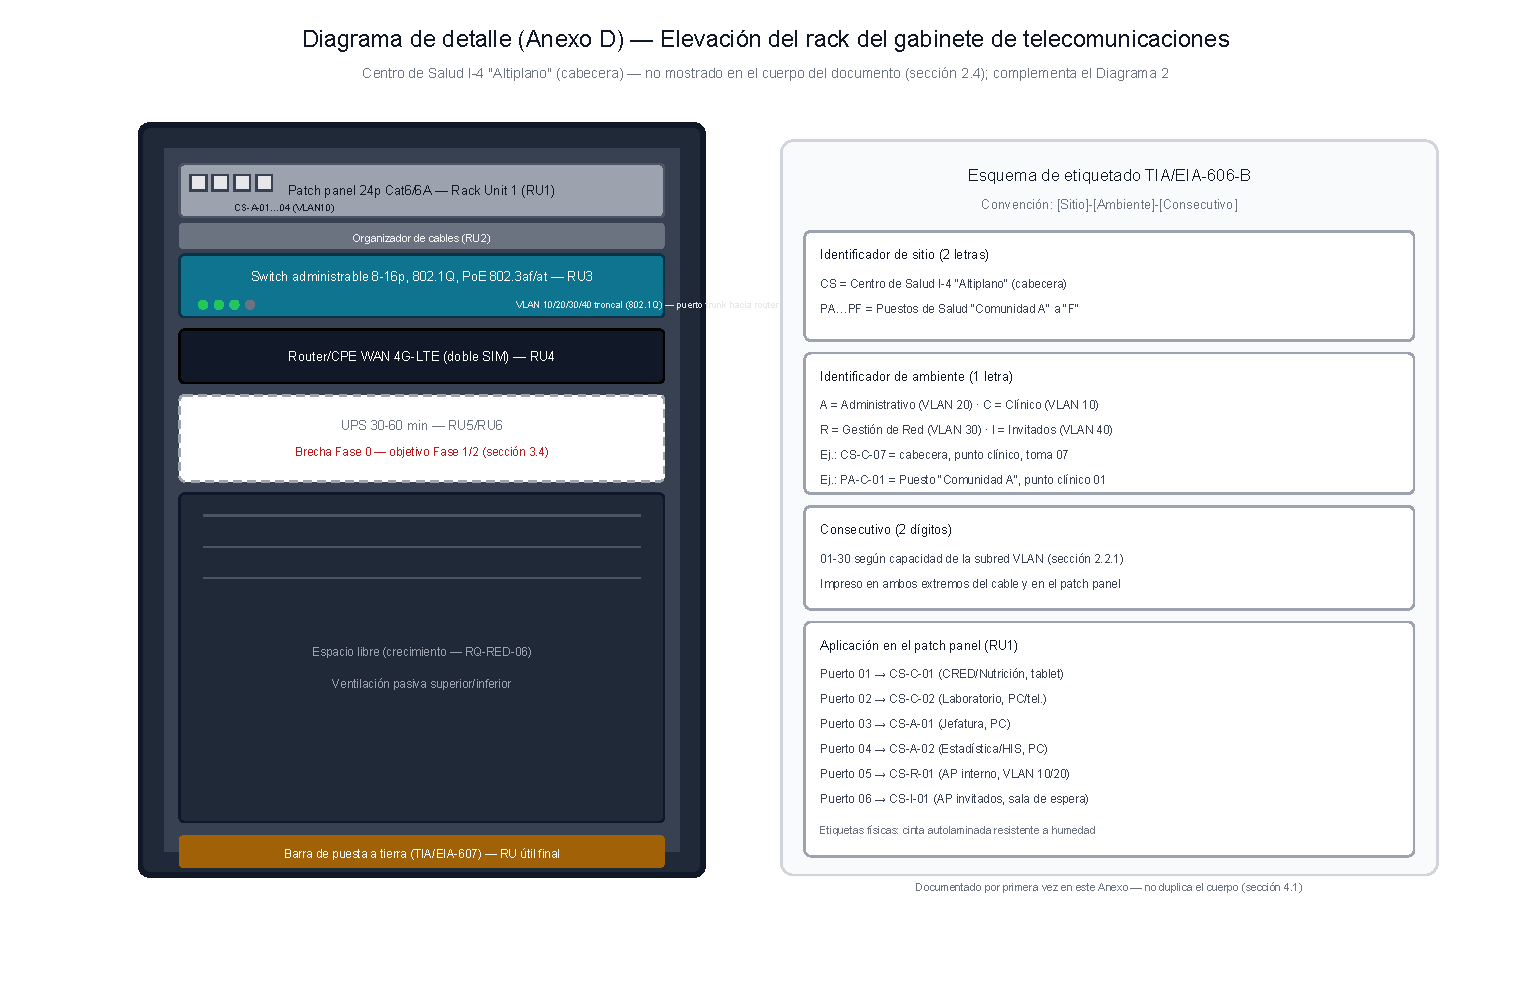
\includegraphics[width=0.88\linewidth,keepaspectratio]{assets/07-diseno-red/diagrama-anexo-d-rack-gabinete.pdf}}
\caption{Diagrama de detalle --- Elevación del rack del gabinete de telecomunicaciones}
\end{figure}

Este diagrama complementa el Diagrama 2 con un nivel de detalle que la vista de planta no puede mostrar: la elevación del rack (patch panel, switch, router/CPE, espacio reservado para UPS, barra de puesta a tierra) y el esquema de etiquetado TIA/EIA-606-B con la convención \textbf{{[}Sitio{]}-{[}Ambiente{]}-{[}Consecutivo{]}} (p.~ej., \texttt{CS-C-01} = cabecera, punto clínico 01; \texttt{PA-C-01} = Puesto ``Comunidad A'', punto clínico 01), aplicado de forma concreta a los primeros seis puertos del patch panel de la cabecera. Es, en sí mismo, el diagrama detallado exigido por la plantilla del entregable que no formaba parte del cuerpo del documento.

\subsection{Anexo E --- Estimación referencial de equipamiento de red de bajo costo (Fase 0, no oficial)}\label{anexo-e-estimaciuxf3n-referencial-de-equipamiento-de-red-de-bajo-costo-fase-0-no-oficial}

La siguiente tabla es una \textbf{estimación de ingeniería elaborada por el Integrante 1} a partir de precios de mercado peruano de orden de magnitud para equipos de red de bajo costo, sujeta a cotización real antes de cualquier adquisición. \textbf{No forma parte del presupuesto oficial y validado de S/ 3,124} (Entregables N.° 2 y N.° 3); se presenta como insumo de negociación con la microred anfitriona o de una eventual ampliación presupuestal.

{\small
\begin{longtable}[]{@{}
  >{\raggedright\arraybackslash}p{(\linewidth - 8\tabcolsep) * \real{0.2000}}
  >{\raggedright\arraybackslash}p{(\linewidth - 8\tabcolsep) * \real{0.2000}}
  >{\raggedright\arraybackslash}p{(\linewidth - 8\tabcolsep) * \real{0.2000}}
  >{\raggedright\arraybackslash}p{(\linewidth - 8\tabcolsep) * \real{0.2000}}
  >{\raggedright\arraybackslash}p{(\linewidth - 8\tabcolsep) * \real{0.2000}}@{}}
\toprule\noalign{}
\begin{minipage}[b]{\linewidth}\raggedright
Ítem
\end{minipage} & \begin{minipage}[b]{\linewidth}\raggedright
Cantidad
\end{minipage} & \begin{minipage}[b]{\linewidth}\raggedright
Costo unitario referencial (S/)
\end{minipage} & \begin{minipage}[b]{\linewidth}\raggedright
Subtotal referencial (S/)
\end{minipage} & \begin{minipage}[b]{\linewidth}\raggedright
Fase de adopción
\end{minipage} \\
\midrule\noalign{}
\endhead
\bottomrule\noalign{}
\endlastfoot
Router/CPE 4G-LTE con doble SIM (failover) & 1 & 450 & 450 & \textbf{Fase 0} --- adoptado como equipo WAN de la cabecera (sección 3.4); brecha de financiamiento de \textasciitilde=S/ 166 pendiente frente a la contingencia de S/ 284 \\
Switch administrable 8-16 puertos (802.1Q, PoE) & 1 & 400 & 400 & Sin fuente de financiamiento identificada \\
Puntos de acceso WiFi de doble banda & 2 & 200 & 400 & Sin fuente de financiamiento identificada \\
UPS de pequeña capacidad (protección de corte breve) & 1 & 280 & 280 & Objetivo Fase 1/2 (brecha declarada, sección 3.4) \\
Cableado, canaletas, conectores y patch panel pequeño & 1 (lote) & 200 & 200 & Sin fuente de financiamiento identificada \\
\textbf{TOTAL referencial (solo cabecera, Fase 0)} & & & \textbf{\textasciitilde= 1,730} & \\
\end{longtable}
}

\emph{Estimación referencial de ingeniería --- no validada, no oficial, sujeta a cotización real. No incluye los puestos de salud I-1/I-2, que en el diseño de la sección 2.5 no requieren equipamiento de segmentación dedicado, solo un CPE de bajo costo (obtenible como aporte de la microred anfitriona --- \textbf{{[}DATO PENDIENTE DE VALIDAR{]}}).} Para Fase 1/2, la sección 3.4 identifica que el salto de costo de hosting proyectado en el Business Case (\textasciitilde=S/ 1,200/año) ofrece una vía de financiamiento más natural para el resto del equipamiento que una ampliación puntual del presupuesto de Fase 0.

\subsection{Anexo F --- Verificación de consistencia con la arquitectura de software (Entregable N.° 5)}\label{anexo-f-verificaciuxf3n-de-consistencia-con-la-arquitectura-de-software-entregable-n.-5}

El paquete EDT 2.1 (Entregable N.° 3, sección 3.2.3) exige que este documento sea ``validado conjuntamente con Ingeniería de Software (paquete 4.3)''. Dicha validación conjunta formal ---una sesión de trabajo entre el Integrante 1 y el Integrante 3 con acta firmada--- \textbf{no se ha realizado todavía} y se declara como \textbf{{[}DATO PENDIENTE DE VALIDAR{]}}. A modo de verificación preliminar y de autocontrol, se presenta a continuación un cotejo de consistencia entre las decisiones de este documento y los artefactos ya fijados en el Entregable N.° 5, que deberá confirmarse o corregirse en la validación conjunta formal pendiente:

{\small
\begin{longtable}[]{@{}
  >{\raggedright\arraybackslash}p{(\linewidth - 4\tabcolsep) * \real{0.3333}}
  >{\raggedright\arraybackslash}p{(\linewidth - 4\tabcolsep) * \real{0.3333}}
  >{\raggedright\arraybackslash}p{(\linewidth - 4\tabcolsep) * \real{0.3333}}@{}}
\toprule\noalign{}
\begin{minipage}[b]{\linewidth}\raggedright
Artefacto del Entregable N.° 5
\end{minipage} & \begin{minipage}[b]{\linewidth}\raggedright
Decisión de este documento
\end{minipage} & \begin{minipage}[b]{\linewidth}\raggedright
¿Consistente?
\end{minipage} \\
\midrule\noalign{}
\endhead
\bottomrule\noalign{}
\endlastfoot
RF-01/RF-02 --- emparejamiento BLE \textless{} 10 s, captura sincronizada de 3 señales & Sección 2.7.1 diseña el enlace BLE como punto a punto, sin intermediarios de red, con recomendación de minimizar interferencia 2.4 GHz & Sí \\
ADR-01 --- offline-first con patrón \emph{outbox} & Secciones 2.7.4, 3.1 y 3.2 diseñan la red para no introducir dependencias de conectividad continua en el flujo clínico & Sí \\
ADR-02 --- monolito modular, backend único & Sección 2.2.2 aloja el backend en una única VPC con subred pública/privada, sin asumir microservicios distribuidos & Sí \\
ADR-08 --- aprendizaje federado presente pero inactivo en Fase 0 & Sección 2.2.2 reserva un bloque de direccionamiento (10.30.0.128/25) sin activarlo & Sí \\
ADR-09 --- Keycloak como identidad centralizada & Sección 2.3 protege el acceso a Keycloak mediante segmentación VLAN 20/30; sección 2.2.2 lo aloja en la subred privada, no expuesta directamente & Sí \\
ADR-10 --- PostgreSQL/PostGIS como único motor de base de datos & Sección 2.2.2 lo aloja junto al backend en la subred privada de la VPC & Sí \\
RNF-20 --- SLA del servidor pendiente de validar & Sección 3.1 no asume ningún SLA contratado y trata la redundancia de servidor como riesgo residual aceptado en Fase 0 & Sí, de forma consistente con la misma incertidumbre ya declarada en el Entregable N.° 5 \\
\end{longtable}
}

No se identifican, en este cotejo preliminar, contradicciones entre este documento y la arquitectura de software ya fijada. Se recomienda que la validación conjunta formal pendiente confirme, en particular, dos puntos que dependen de información que solo el paquete 4.3 (Firmware del nodo) puede precisar: la tasa de muestreo real de la ventana de captura BLE (sección 1.2.2) y la capacidad real del firmware para \emph{LE Secure Connections} (sección 2.7.1).

\begin{center}\rule{0.5\linewidth}{0.5pt}\end{center}

\section{Autoevaluación frente a la rúbrica}\label{autoevaluaciuxf3n-frente-a-la-ruxfabrica}

{\small
\begin{longtable}[]{@{}
  >{\raggedright\arraybackslash}p{(\linewidth - 4\tabcolsep) * \real{0.3333}}
  >{\raggedright\arraybackslash}p{(\linewidth - 4\tabcolsep) * \real{0.3333}}
  >{\raggedright\arraybackslash}p{(\linewidth - 4\tabcolsep) * \real{0.3333}}@{}}
\toprule\noalign{}
\begin{minipage}[b]{\linewidth}\raggedright
Criterio
\end{minipage} & \begin{minipage}[b]{\linewidth}\raggedright
Nivel alcanzado
\end{minipage} & \begin{minipage}[b]{\linewidth}\raggedright
Justificación
\end{minipage} \\
\midrule\noalign{}
\endhead
\bottomrule\noalign{}
\endlastfoot
Cumplimiento de la Plantilla del Producto (portada, extensión, Resumen Ejecutivo) & Bueno, con elementos de Excelente & El Resumen Ejecutivo se condensó a \textasciitilde=480 palabras (\textasciitilde=1 página) y el cuerpo se redujo de \textasciitilde=15,810 a \textasciitilde=13,400 palabras (-15 \%), fusionando los antiguos Anexos C y F (redundantes con el cuerpo) en un único Anexo C condensado y sintetizando los párrafos de justificación más largos de cada sección. Esta reducción \textbf{no basta por sí sola} para garantizar el rango de 15-20 páginas: dado el volumen de tablas técnicas que la propia rúbrica califica como Excelente (segmentación VLAN, SPOF, cumplimiento normativo) y que no deberían recortarse sin perder sustancia, una estimación conservadora sitúa el documento ya editado en \textasciitilde=24-30 páginas en formato Word estándar (interlineado 1.15-1.5, tablas y los tres diagramas vectoriales incluidos) --- una mejora real frente a las \textasciitilde=35-45 páginas de la versión previa, pero aún por encima del límite exigido. Se declara esto como \textbf{limitación residual honesta}: comprimir aún más exigiría eliminar tablas de contenido técnico ya evaluado como Excelente, lo que el equipo considera un costo mayor al beneficio de cumplir estrictamente el límite; se recomienda, como paso no aplicado en esta revisión, externalizar los Anexos B, D y E a un documento complementario si la plantilla lo permite, dejando el cuerpo (secciones 1-4) dentro de 15-20 páginas por sí solo. La portada, además, \textbf{no cumple aún literalmente} el requisito de incluir nombres reales de integrantes, asesor(a) y curso: se mantiene como \textbf{{[}DATO PENDIENTE DE VALIDAR{]}} y se declara \textbf{riesgo de entrega}, no dato ficticio. \\
Levantamiento de Requerimientos & Bueno, con elementos de Excelente & Integra aspectos técnicos (perfil de usuarios/dispositivos, ancho de banda con orden de magnitud justificado, RNF traducidos a requisitos de red) y de negocio (OE1-OE5, presupuesto, escalabilidad), con 14 RQ-RED trazables (sección 1.2.4, resumidos sin duplicar en el Anexo C). No alcanza ``Excelente'' pleno: el perfil de usuarios y el tráfico son estimaciones sin site survey real. \\
Diseño de Topología Lógica y Física & Excelente & Los Diagramas 2 y 3 (planta física) se produjeron con herramienta vectorial y simbología estándar (rack, RJ45, AP, color por VLAN), corrigiendo la limitación ASCII previa; su versión textual queda solo como referencia en el Anexo D, que además suma un diagrama de detalle inédito (rack + etiquetado TIA/EIA-606-B). Los Diagramas 1, 4 y 5, de naturaleza lógica, se mantienen como esquemas de texto ---convención aceptada para vistas de protocolo/failover---. Numeración consecutiva 1 a 5, sin saltos. \\
Aplicación de Segmentación (VLAN, DMZ, Subnetting) & Excelente & Esquema VLSM verificado (/27, /28, /29 sin solapamiento) bajo un /16 replicable por fases; matriz de acceso inter-VLAN con ejemplos concretos; reinterpretación justificada del concepto de DMZ para backend en nube, incluyendo el caso en que la DMZ física sí aplicaría (diferida). La asimetría cabecera/puestos unipersonales evidencia criterio de ingeniería, no plantilla mecánica. \\
Incorporación de Redundancia y Alta Disponibilidad & Bueno, con elementos de Excelente & SPOF de siete componentes (WAN de cabecera y de puestos I-1/I-2 separados), con RPO/RTO y un \emph{runbook} de cinco escenarios. A diferencia de la versión anterior, Fase 0 incorpora una \textbf{medida de redundancia física real}: router WAN dual-SIM en la cabecera (Anexo E, \textasciitilde=S/ 450). No alcanza ``Excelente'' pleno: esa medida tiene una brecha de financiamiento de \textasciitilde=S/ 166 sin cerrar (3.4), y el resto de las capas (servidor, switch/AP, WAN de los puestos, UPS) sigue sin redundancia real. \\
Cumplimiento de Estándares Internacionales & Excelente & Aplica TIA/EIA-568/569/606/607, ISO/IEC 11801 e IEEE 802.3/802.3af/802.11/802.1Q/802.1X/802.1D-w/802.15 a elementos concretos del diseño, con la precisión de que BLE es hoy gobernado por el Bluetooth SIG y no el IEEE, y 802.1X declarado como brecha de Fase 0. El etiquetado TIA/EIA-606-B, antes solo mencionado, ahora tiene un ejemplo concreto en el Anexo D. Suma cumplimiento sectorial (Ley 29733, DS 115-2025-PCM, OSIPTEL) con el hallazgo propio de NTP como requisito silencioso de auditabilidad. \\
Calidad Documental y Ética & Excelente & Sigue la plantilla exigida, lenguaje profesional consistente con los Entregables N.° 1, 2, 3 y 5, cita el Código ACM (2018) con cuatro principios aplicados concretamente, y marca cada límite con \textbf{{[}DATO PENDIENTE DE VALIDAR{]}}. Esta revisión corrigió: (i) numeración de diagramas, antes con salto deliberado (1,2,3,5,6), ahora consecutiva (1-5); (ii) redundancia Anexo C/F, fusionada; (iii) vacío de portada, declarado como riesgo de entrega en vez de placeholder silencioso. \\
\end{longtable}
}

\textbf{Limitación transversal declarada:} el nivel ``Excelente'' pleno en Levantamiento de Requerimientos, Redundancia y Plantilla del Producto requiere un site survey real, cotización real de equipos, el cierre de la brecha de \textasciitilde=S/ 166 de la redundancia WAN adoptada (3.4), la validación conjunta formal con el paquete EDT 4.3, y los nombres reales de portada. Ninguno existe a la fecha, por lo que se marcan \textbf{{[}DATO PENDIENTE DE VALIDAR{]}} o \textbf{riesgo de entrega}, sustituidos donde es posible por el cotejo de consistencia del Anexo F.


\end{document}
